
\documentclass{article}

\usepackage{graphicx}

\usepackage[margin=0.5cm]{geometry}
\usepackage{amsmath}
\usepackage{indentfirst}
\usepackage{hyperref}
\usepackage{multirow}
\usepackage{comment}

\newcommand{\cosa}{\cos\hat\alpha}
\newcommand{\size}{0.33\textwidth}
\newcommand{\pt}{p_\text{T}}

\begin{document}

\title{Toy MC generation for 7 and 13 TeV $J\psi$}
\author{Mariana Ara\'ujo (LIP)}
\maketitle

\begin{table}[h!]
\centering
\begin{tabular}{c | c || c | c | c}
Parameter & Value $(\times10^3)$ & Parameter & Value & Dev ($\sigma$) \\
\hline
$N_{J/\psi}$ & $0.0$ & $L_{\text{CMS,7}}$ & $0.950\pm0.013$ & -2.3 \\
$N_{\psi(2S)}$ & $0.0$ & $L_{\text{CMS,13}}$ & $1.163\pm0.015$ & 7.1 \\
$N_{\Upsilon(1S)}$ & $0.0000001327\pm0.0000000022$ & $L_{\text{LHCb,7},J/\psi}$ & $1.000000\pm0.000000$ & 0.000000 \\
$N_{\Upsilon(2S)}$ & $0.0000000678\pm0.0000000012$ & $L_{\text{LHCb,7}}$ & $0.943\pm0.013$ & -3.4 \\
$N_{\Upsilon(3S)}$ & $0.00000003888\pm0.00000000078$ & $L_{\text{LHCb,13}}$ & $0.870\pm0.019$ & -3.3 \\
\hline
& & $f_{\beta2}$ & $(51.7\pm1.1)$\% & 
\end{tabular}
\caption{Results of the normalization fit. $\chi^2/$ndf = 526 / 270.}
\label{t:fit}
\end{table}


\begin{figure}[h!]
\centering
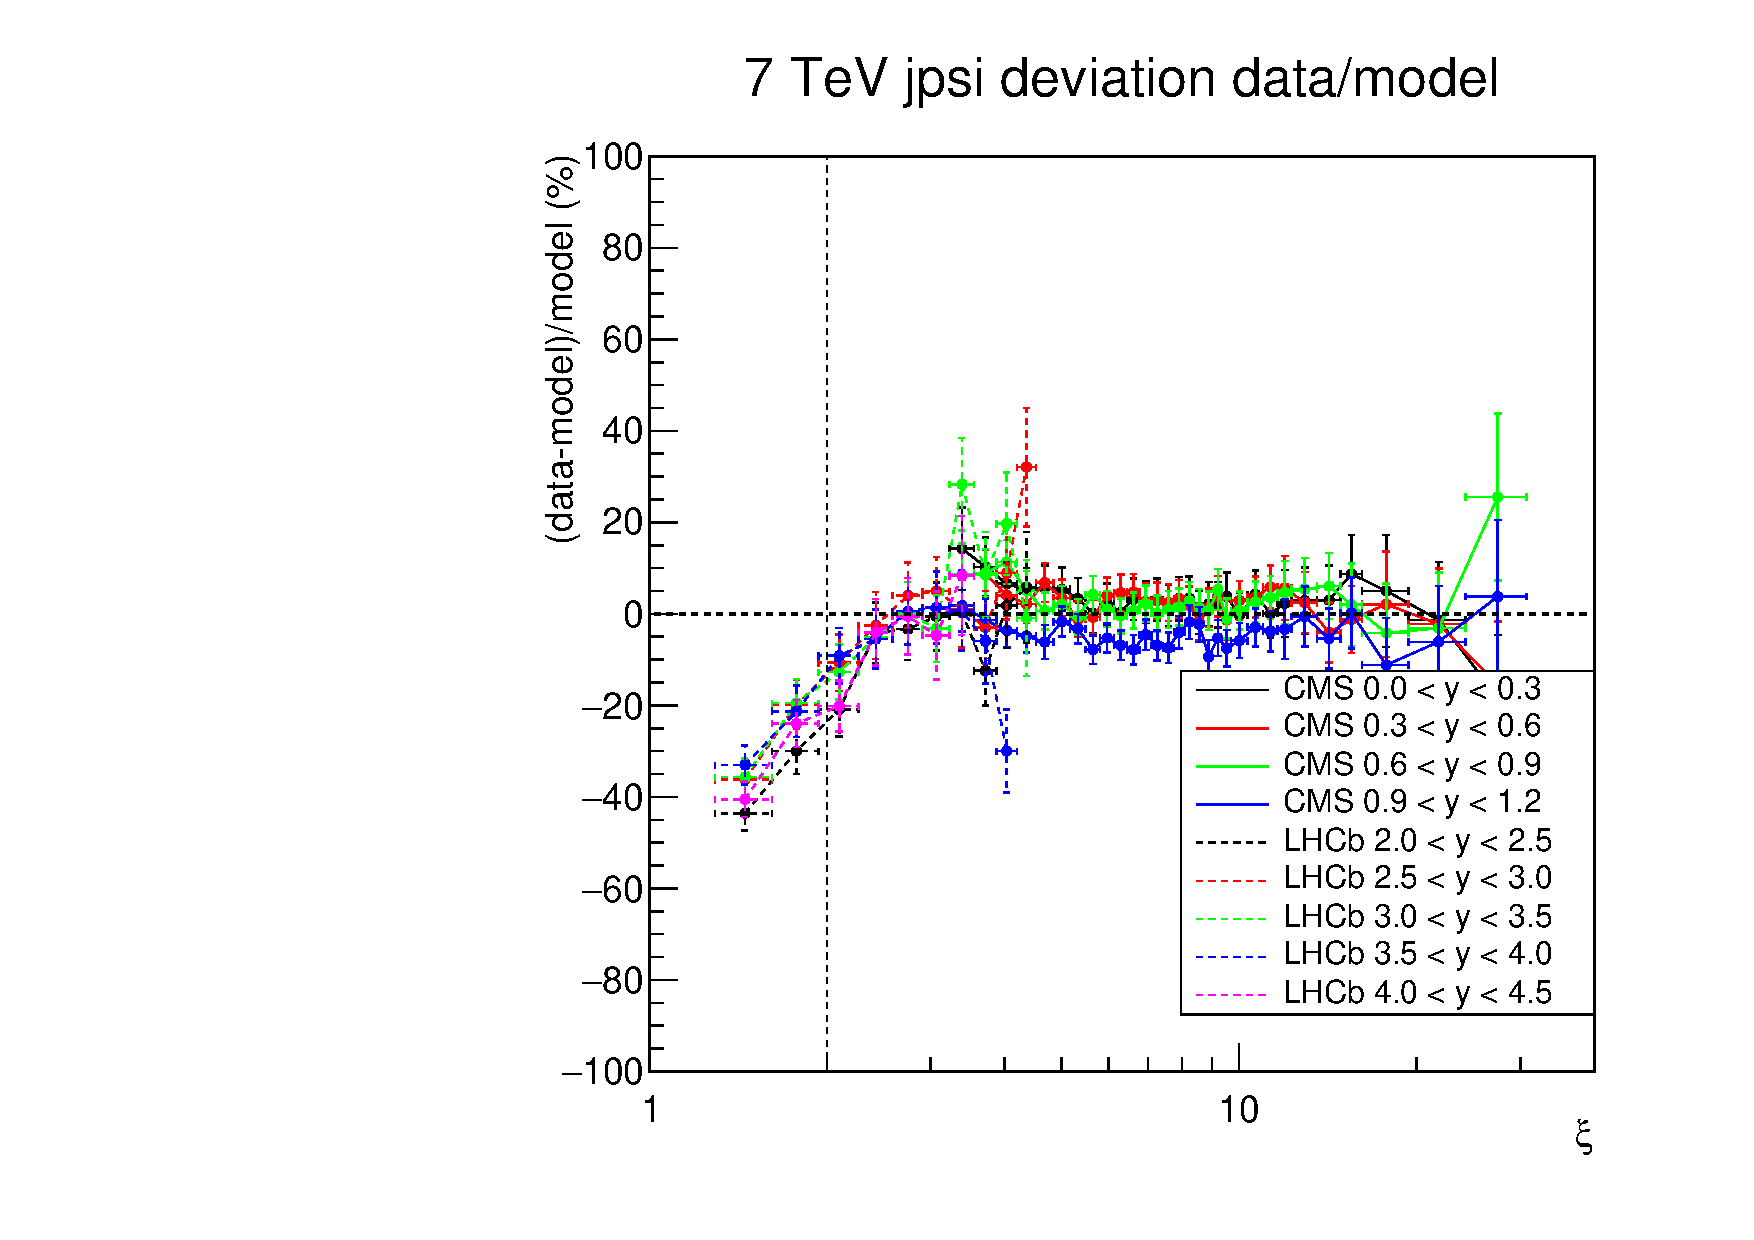
\includegraphics[width = 0.4\textwidth]{xi_devs_jpsi_7.pdf}
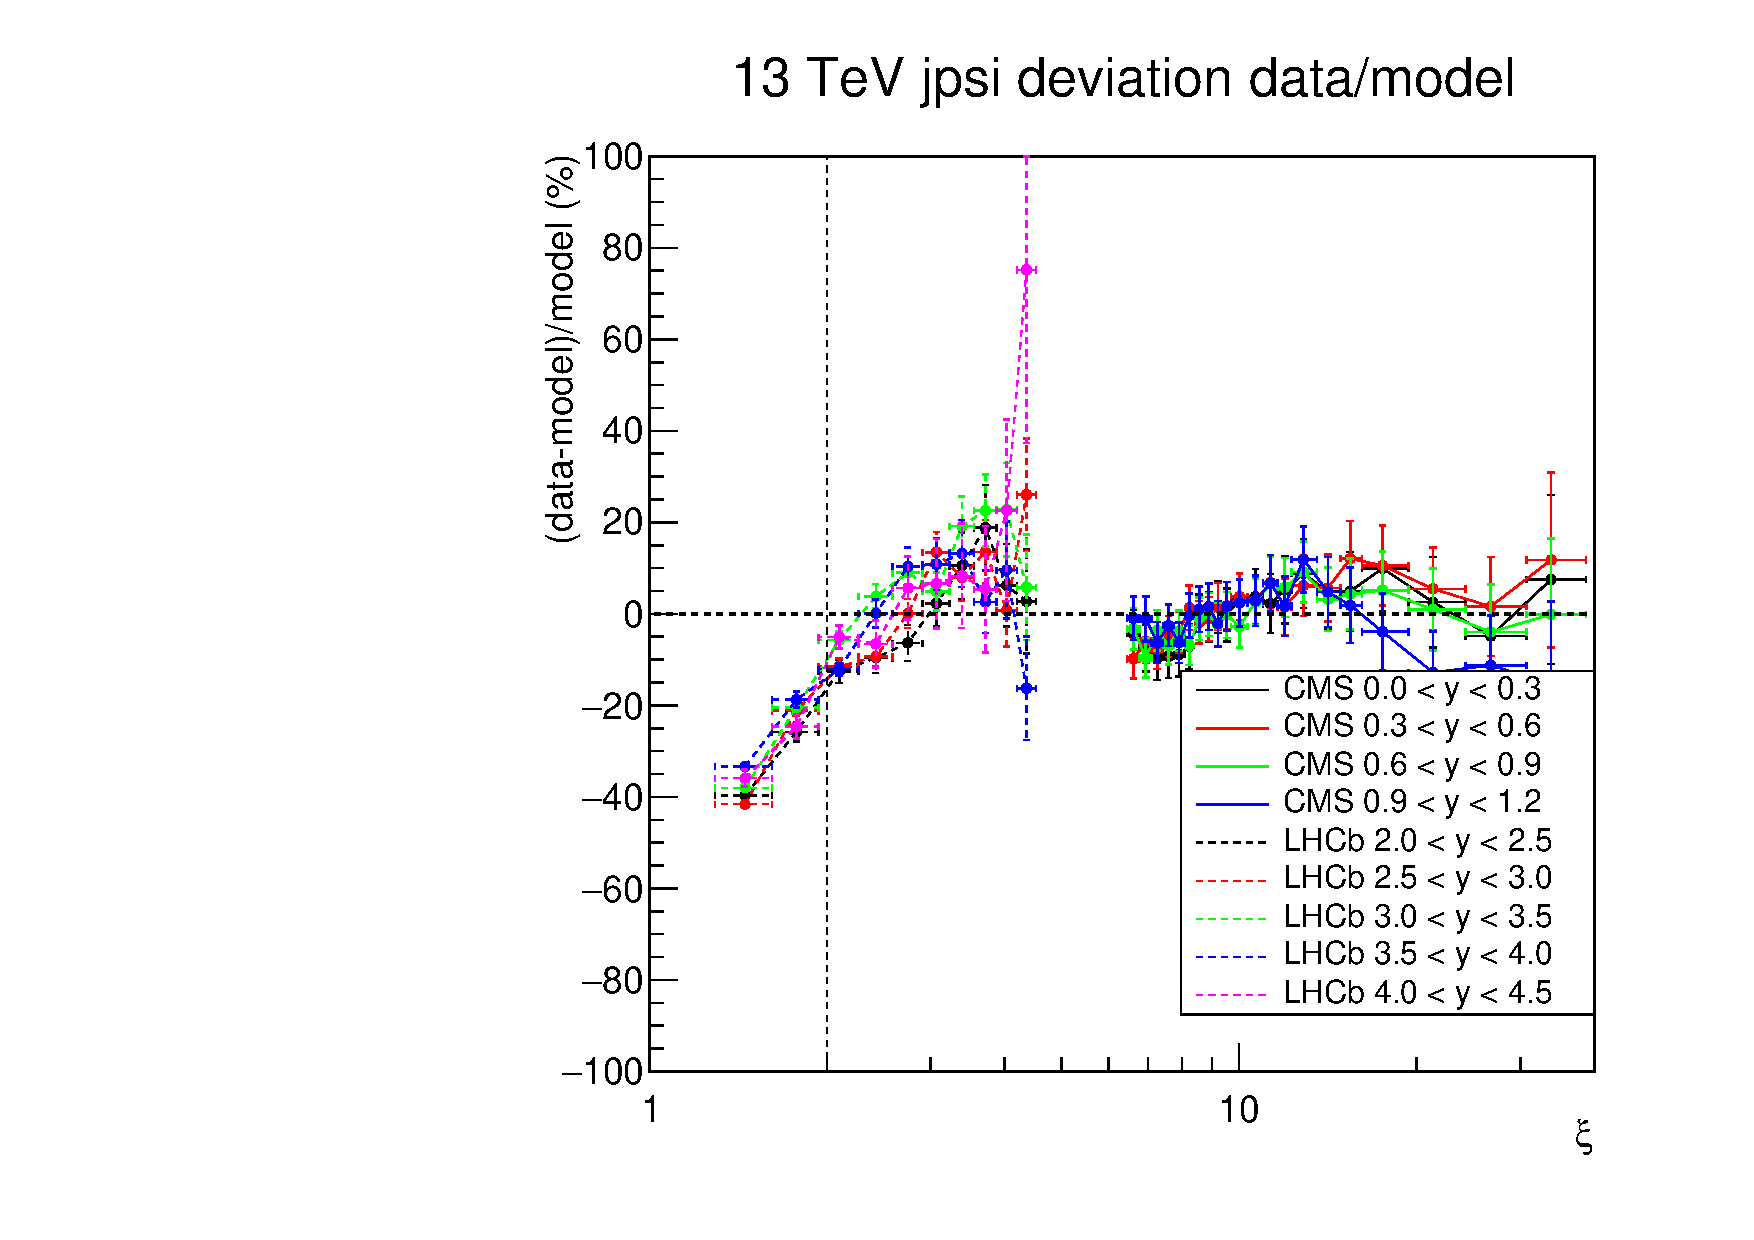
\includegraphics[width = 0.4\textwidth]{xi_devs_jpsi_13.pdf}
\caption{Relative deviations of the fit}\label{f:xi_dev}
\end{figure}

\pagebreak

\begin{figure}[h!]
\centering
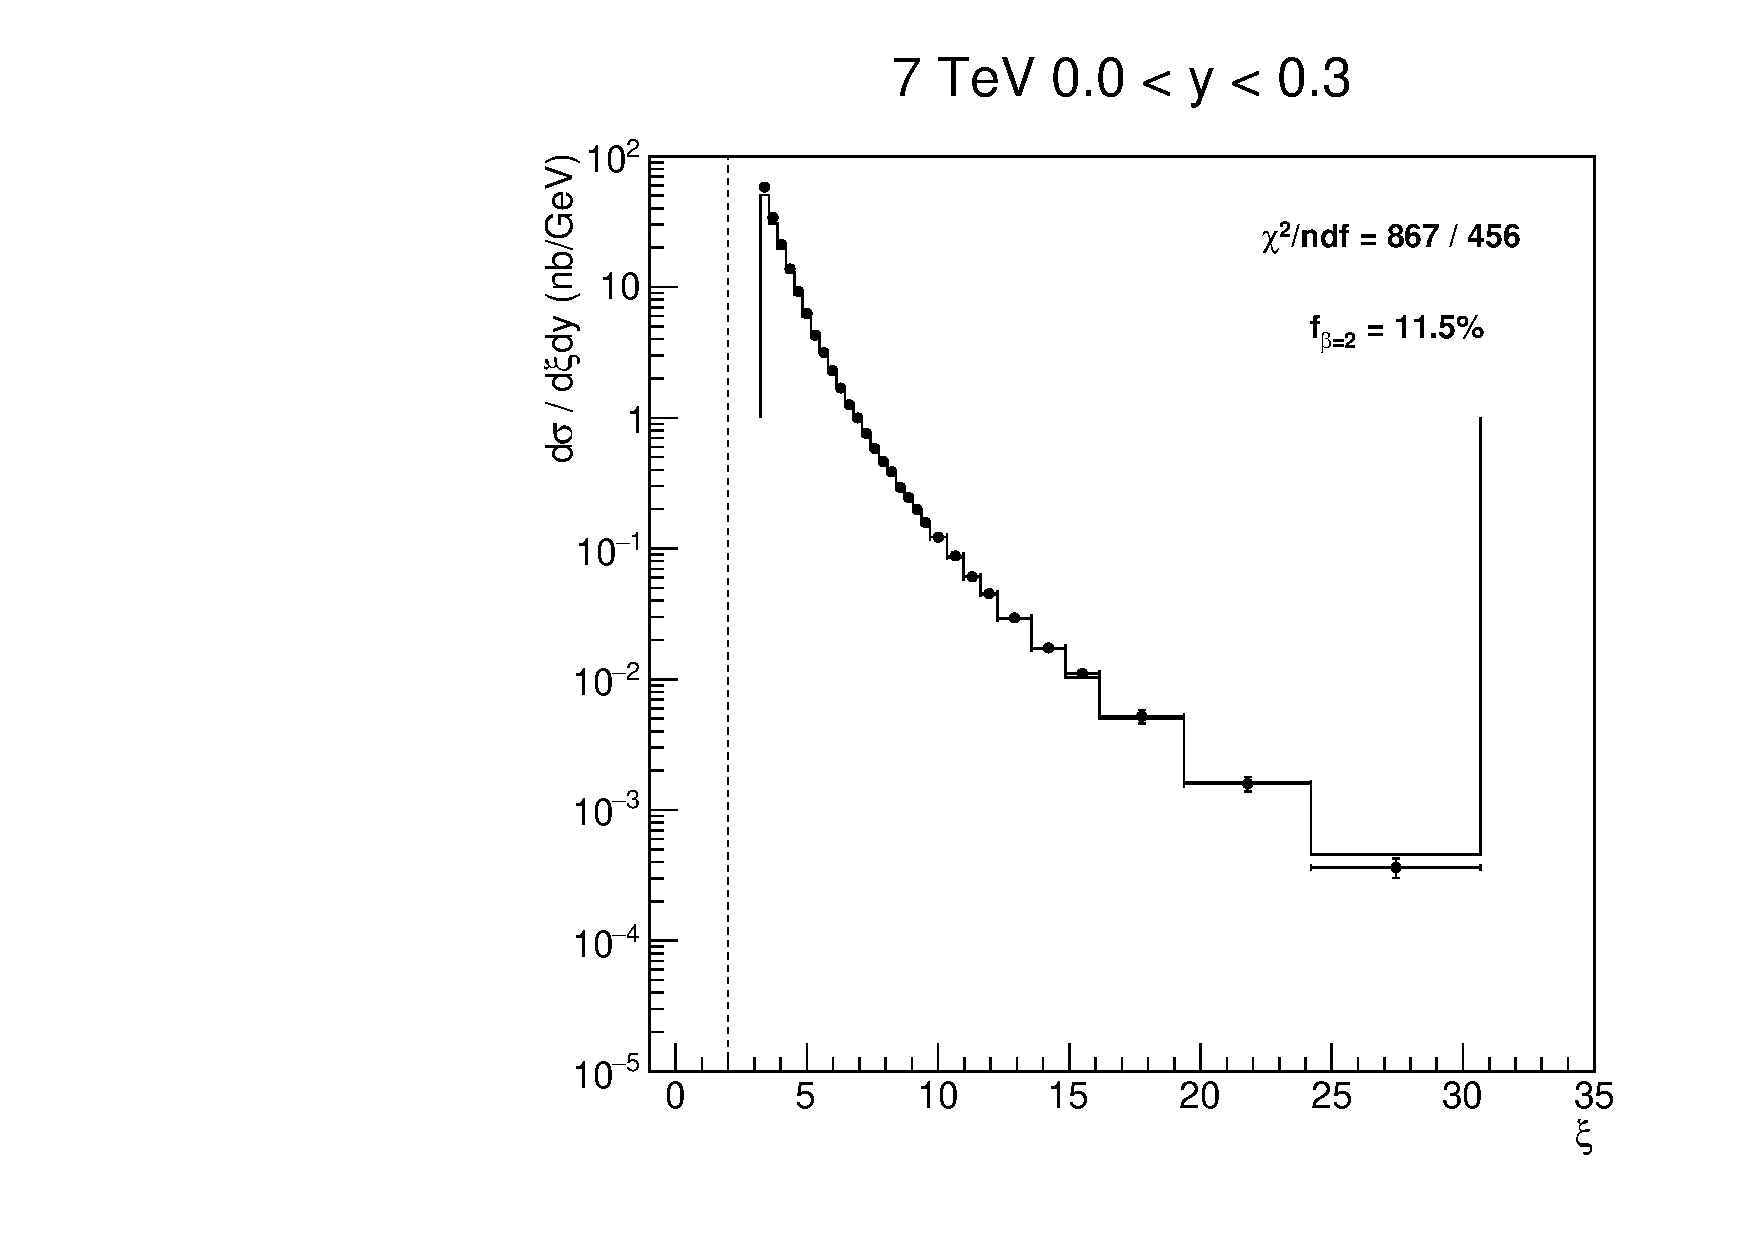
\includegraphics[width = 0.4\textwidth]{xi_7_y1.pdf}
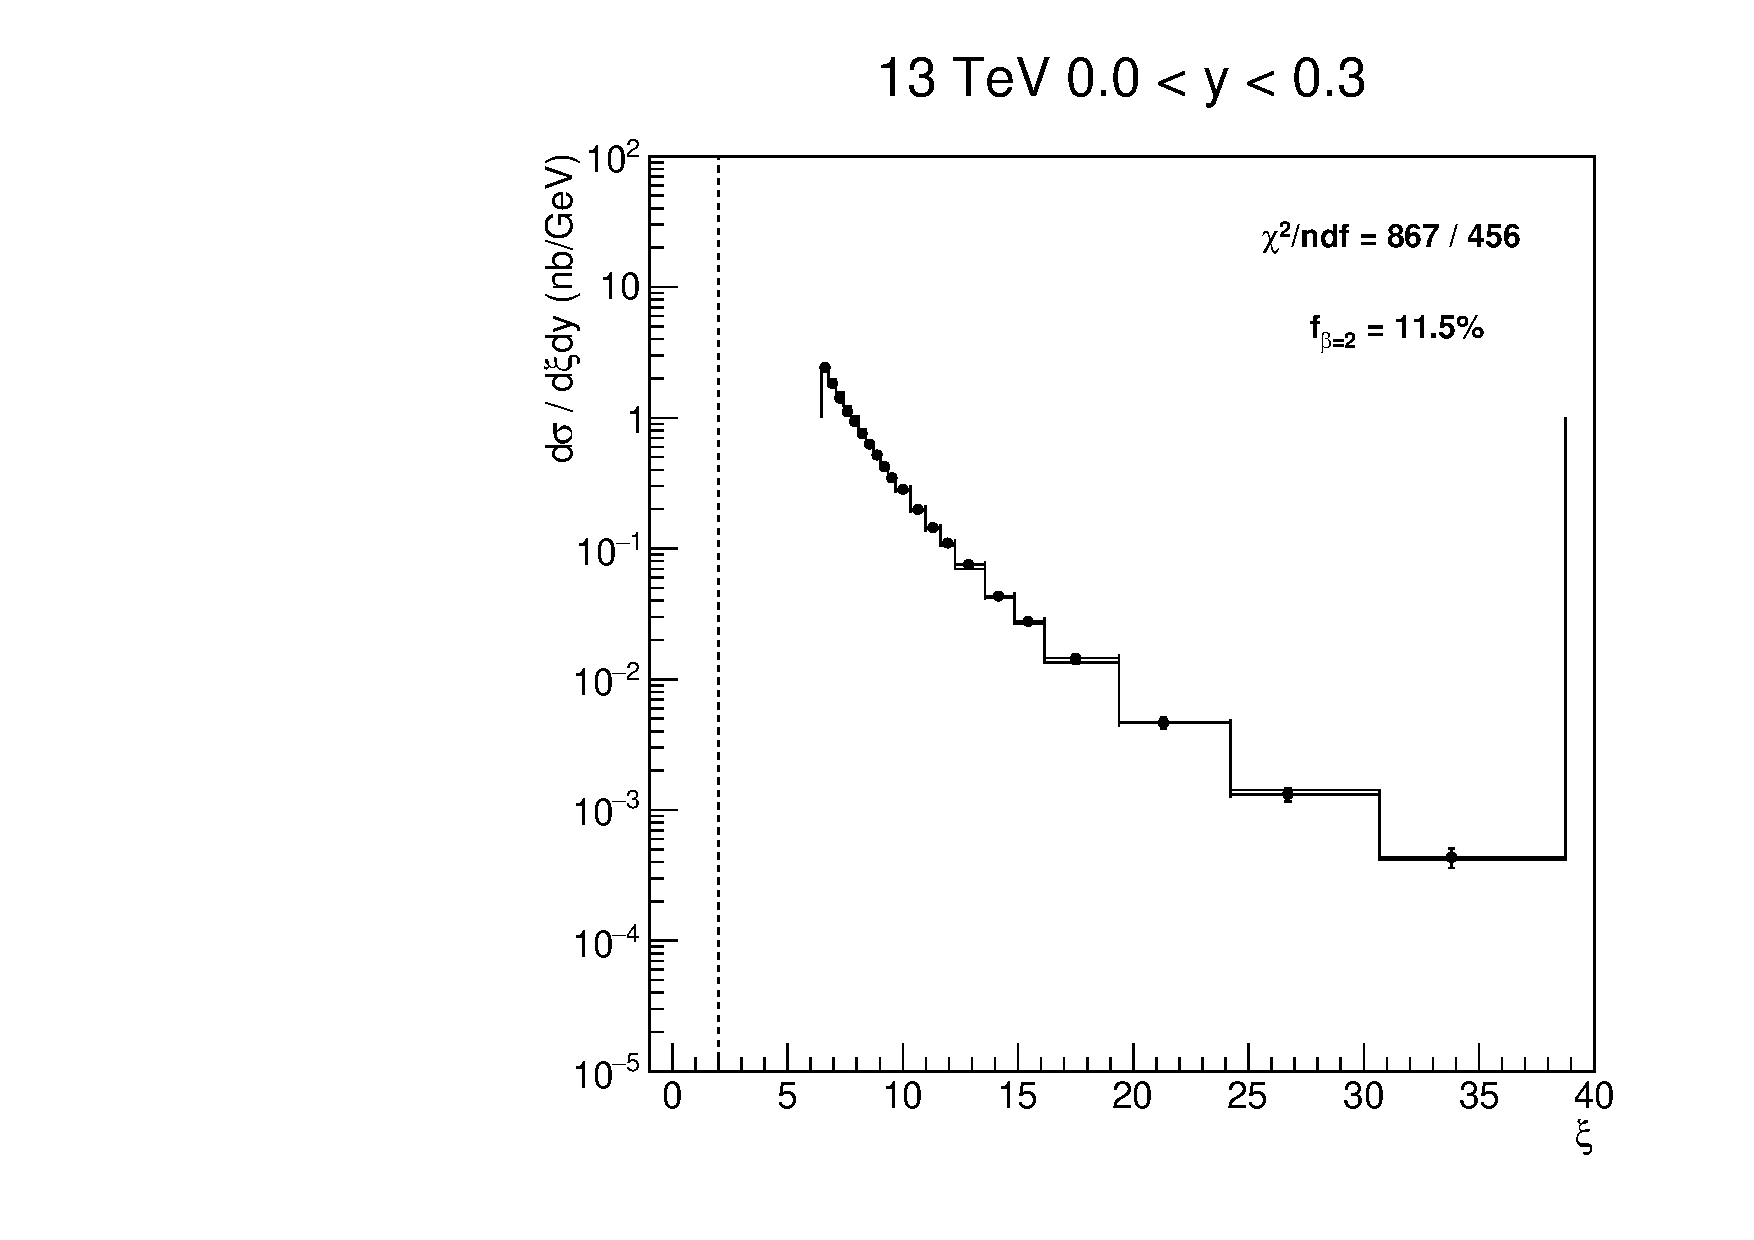
\includegraphics[width = 0.4\textwidth]{xi_13_y1.pdf}

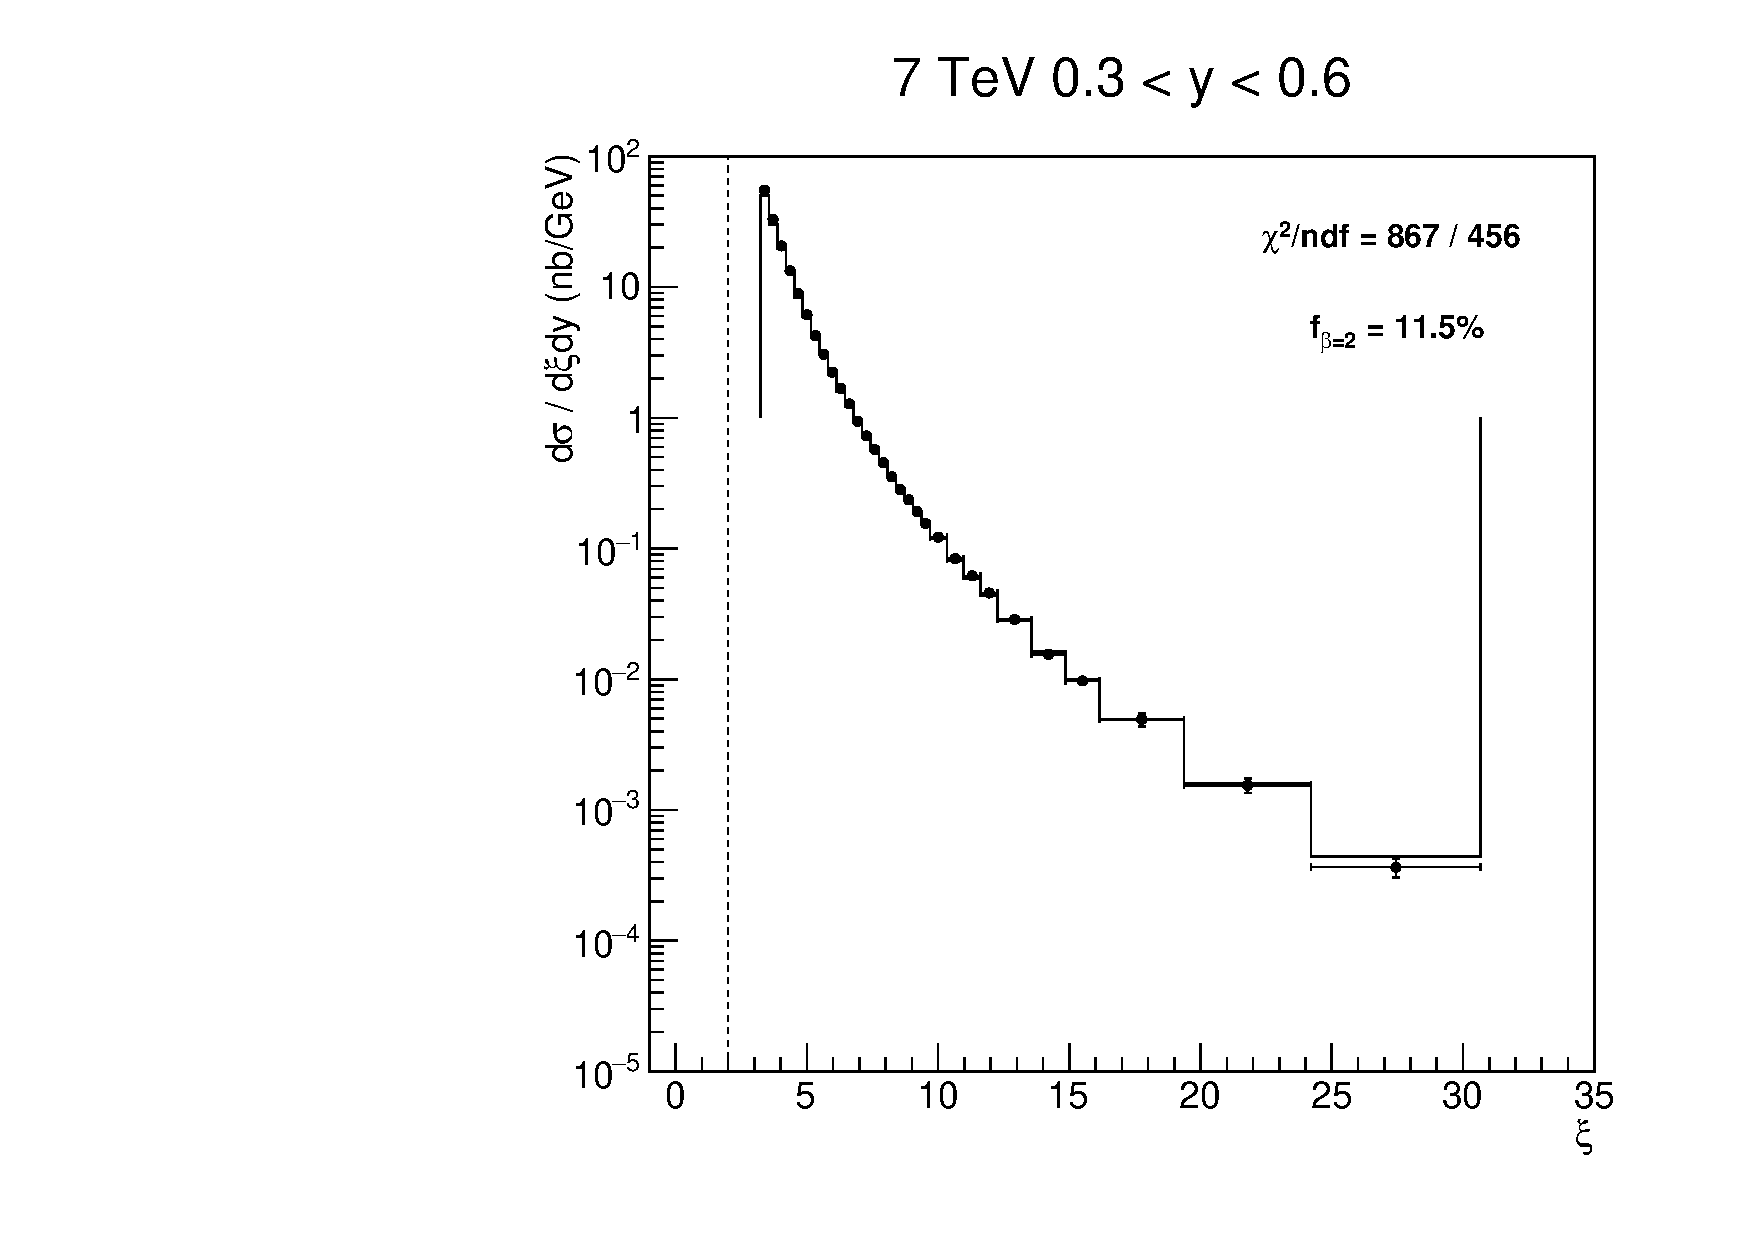
\includegraphics[width = 0.4\textwidth]{xi_7_y2.pdf}
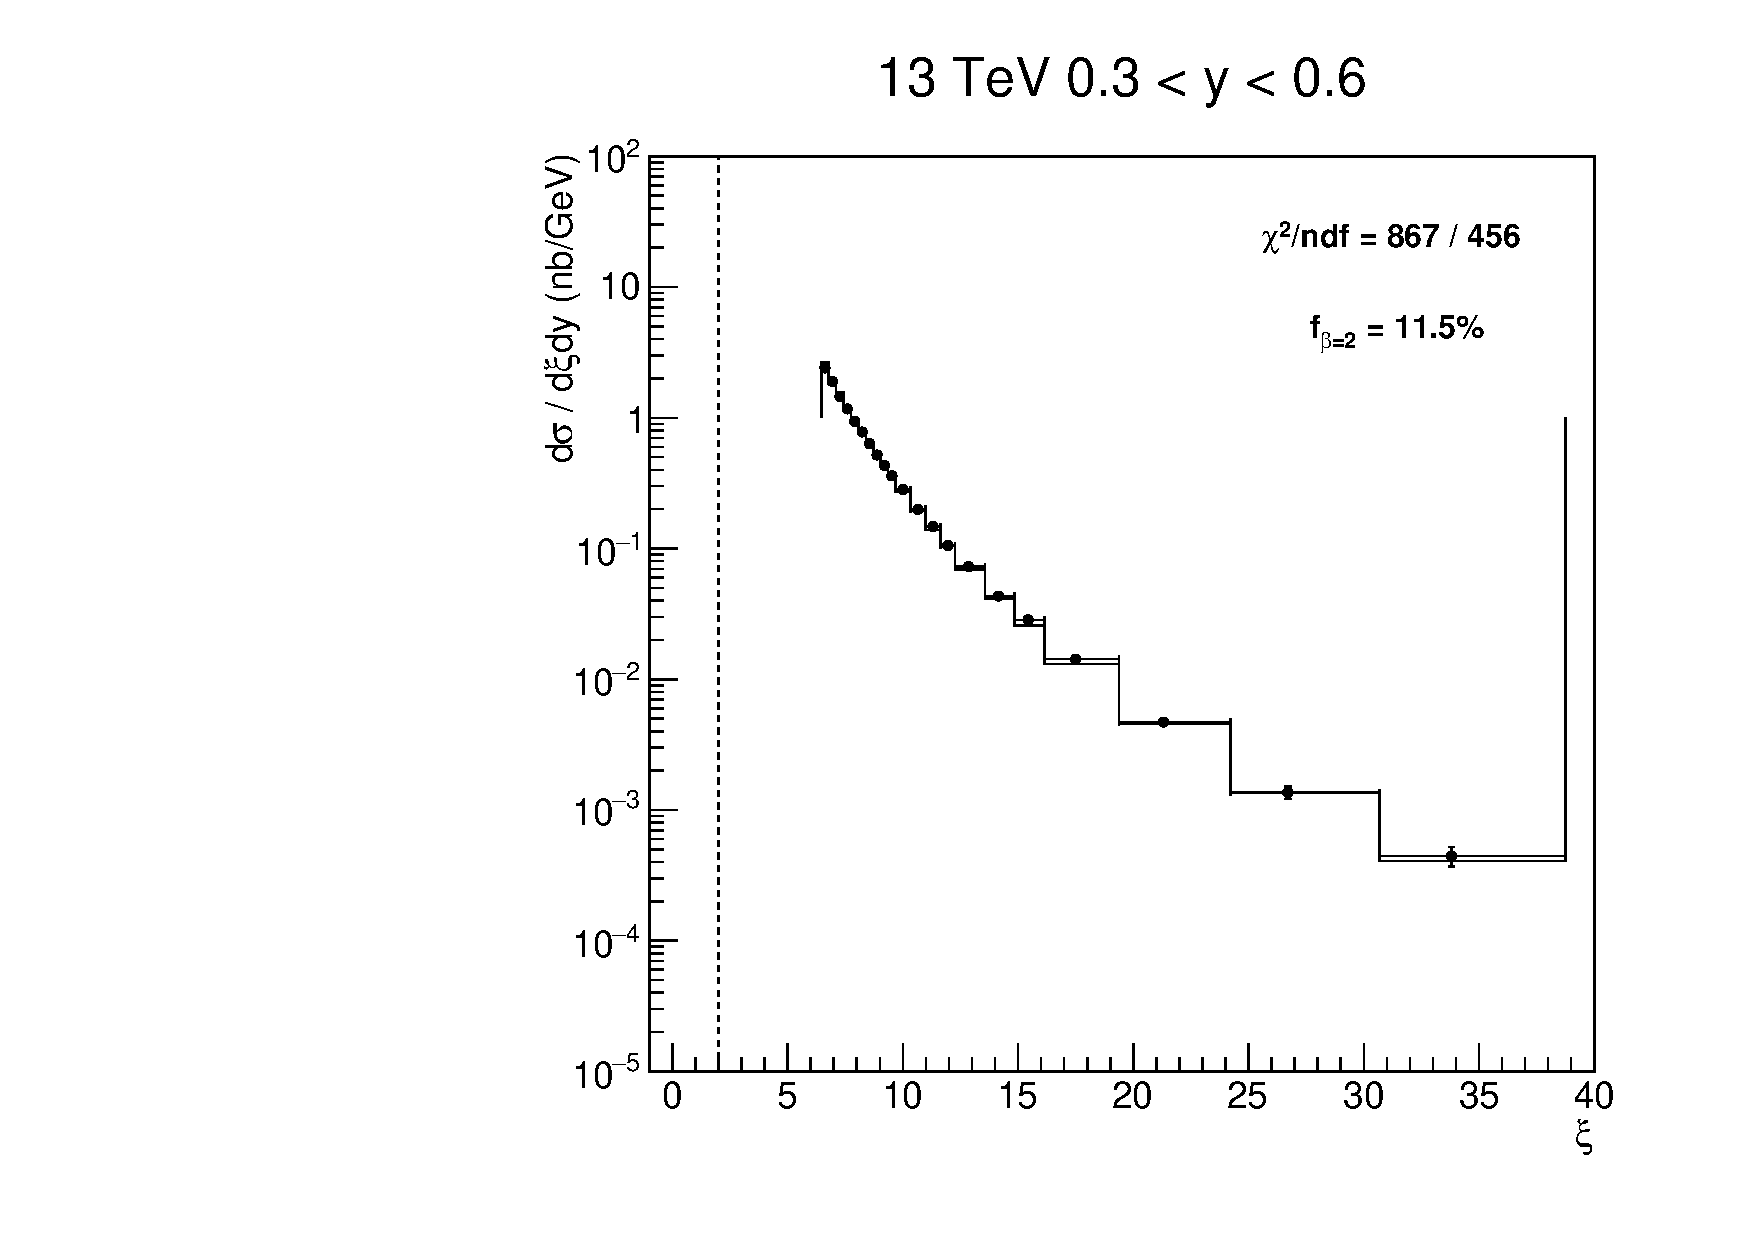
\includegraphics[width = 0.4\textwidth]{xi_13_y2.pdf}

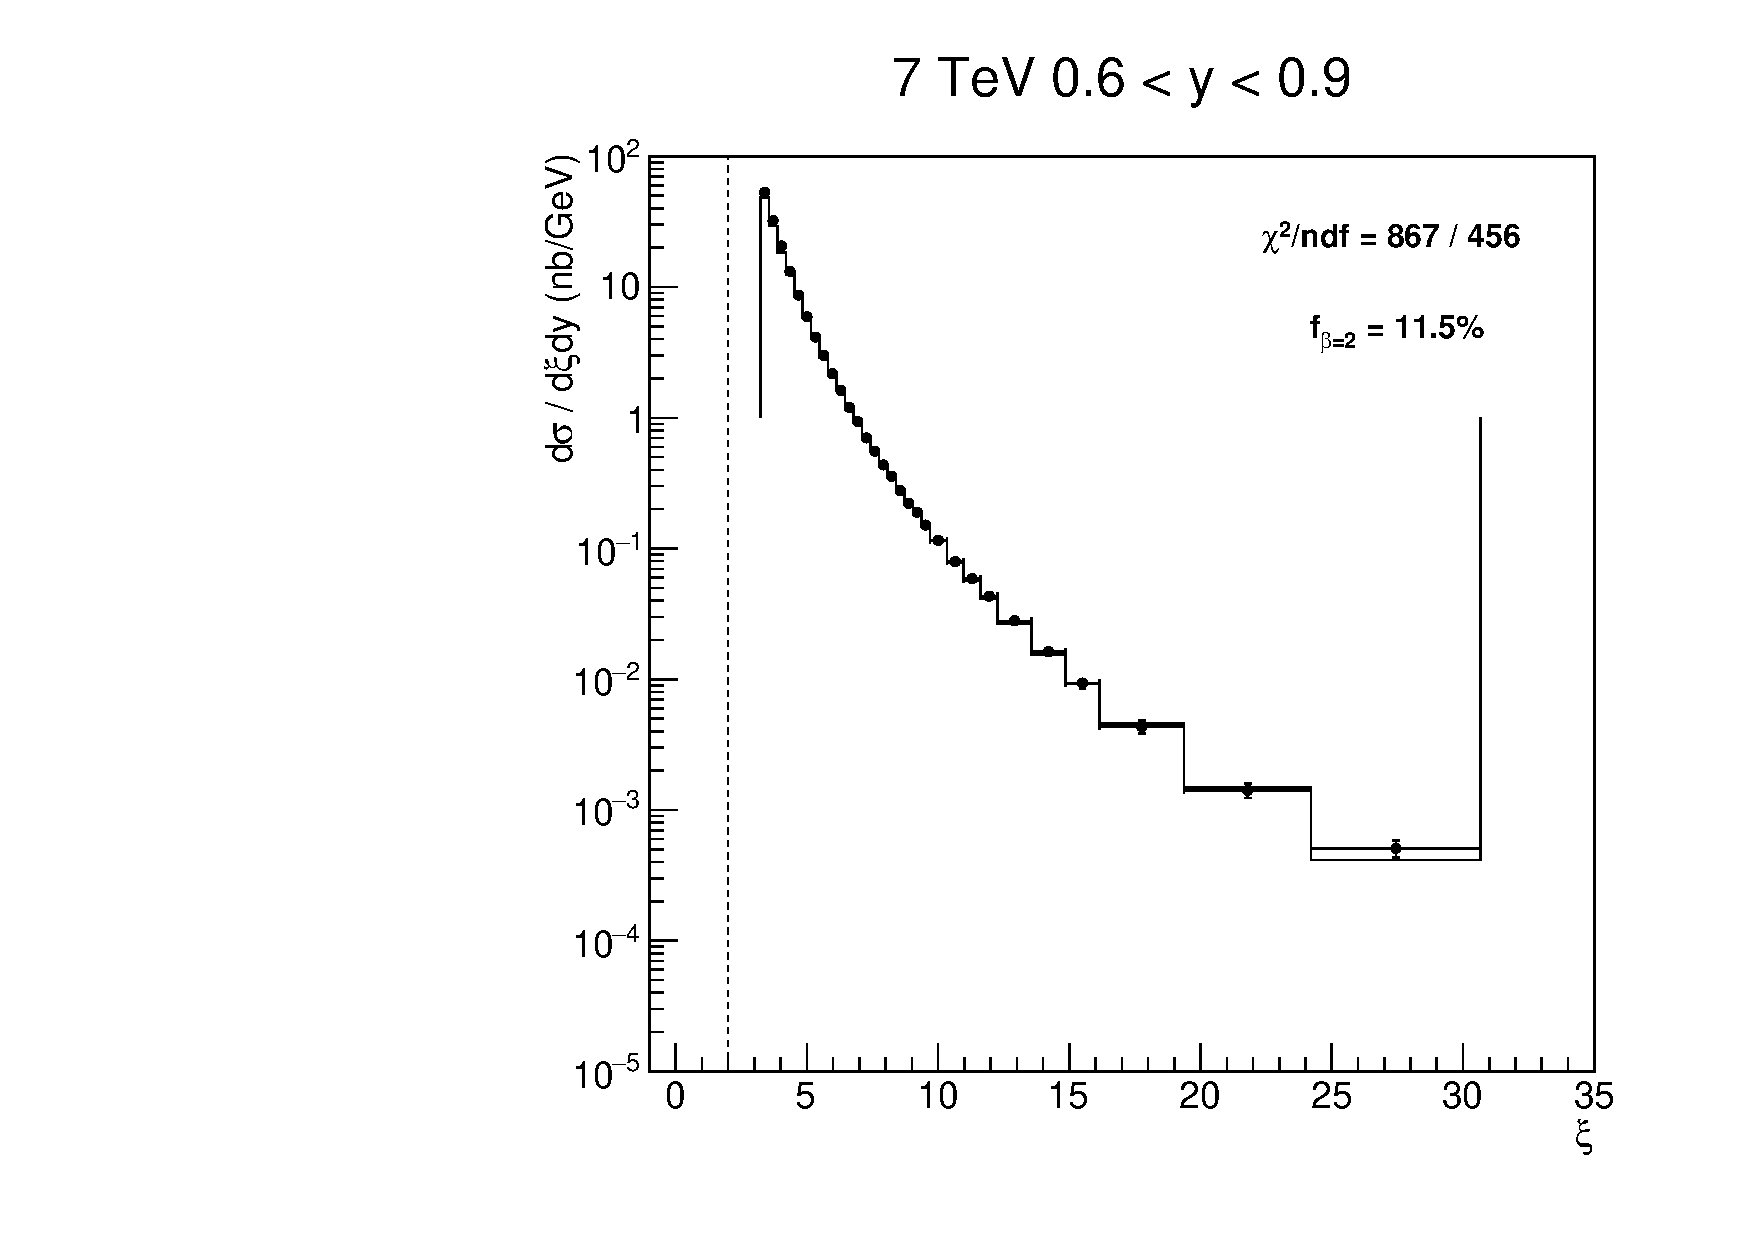
\includegraphics[width = 0.4\textwidth]{xi_7_y3.pdf}
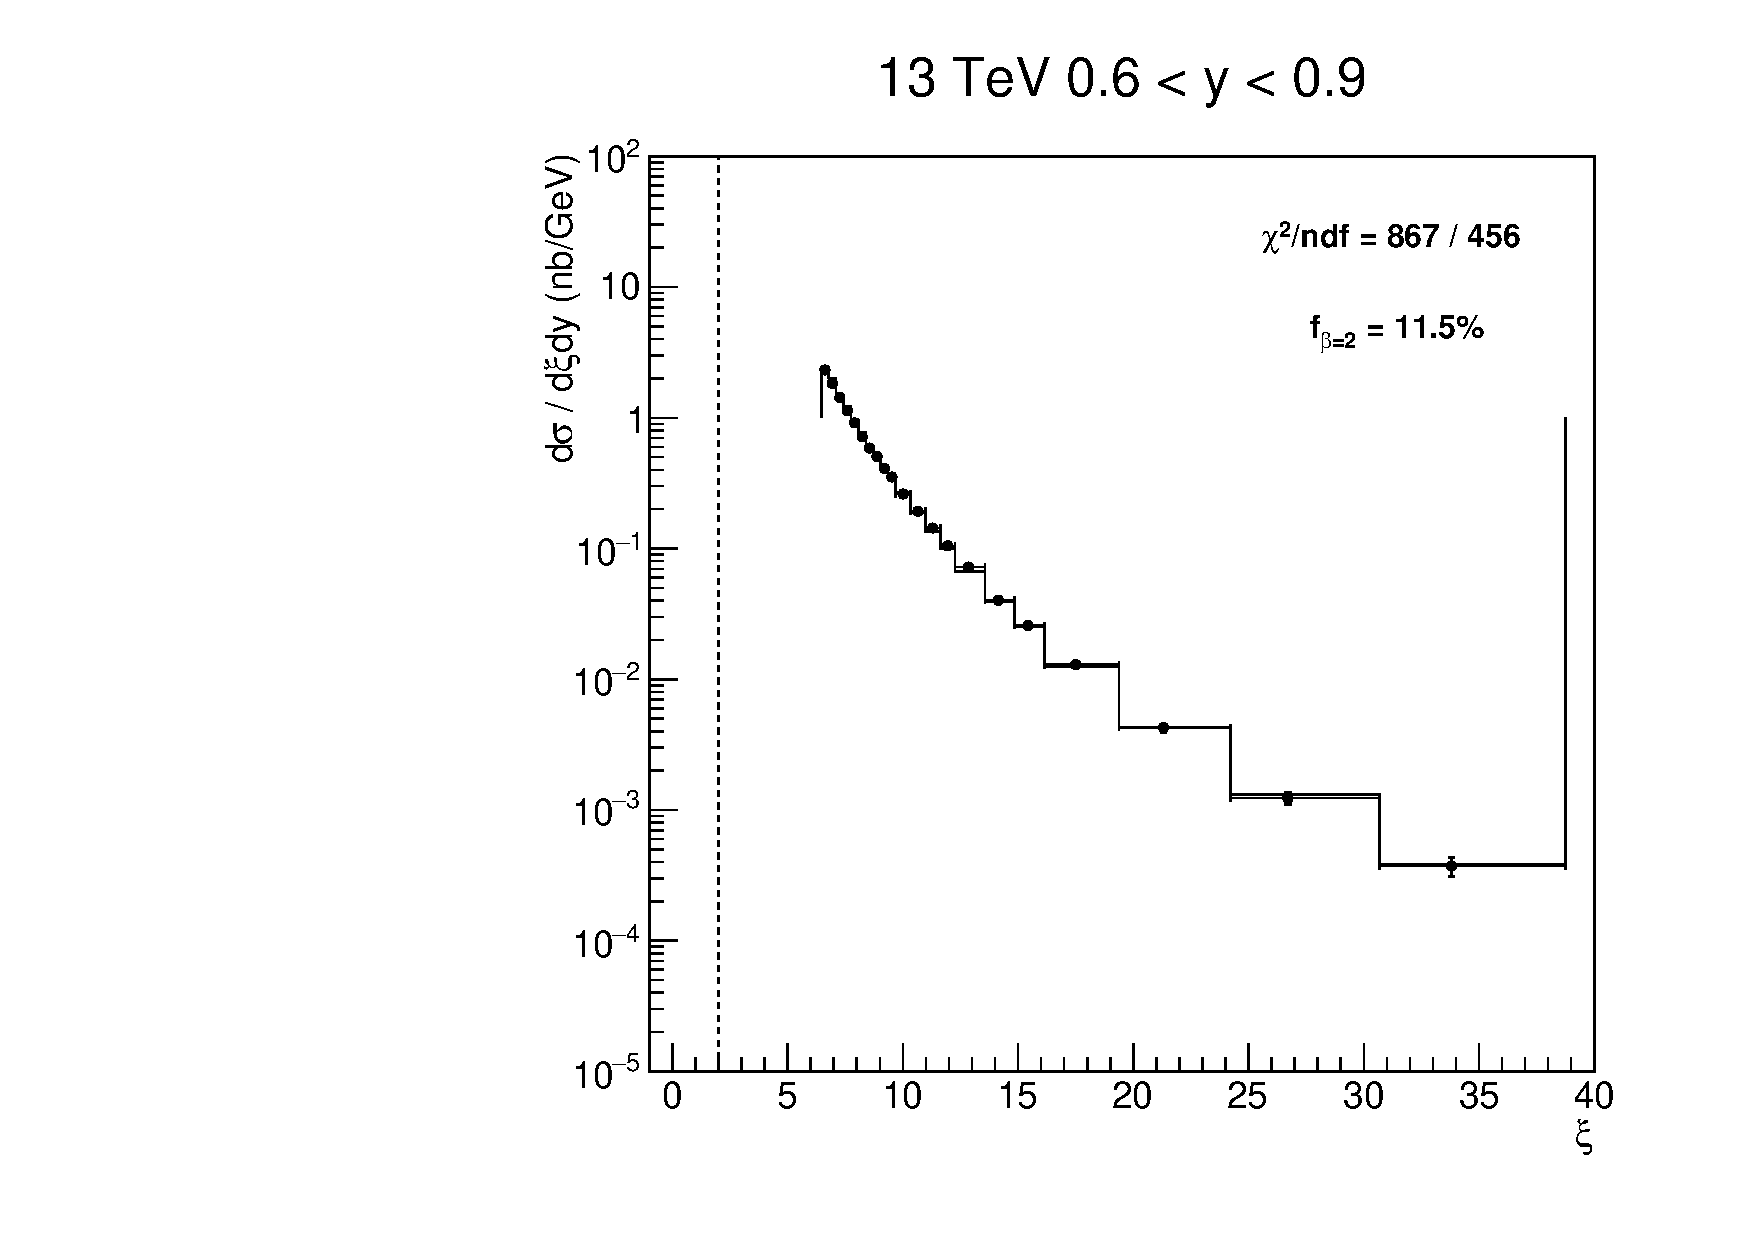
\includegraphics[width = 0.4\textwidth]{xi_13_y3.pdf}
\caption{Comparison between MC $\xi$ distribution and data points in the first three $y$ bins of the data, for 7 TeV (left) and 13 TeV (right).}\label{f:xi_comp_1}
\end{figure}

\clearpage

\begin{figure}[h!]
\centering
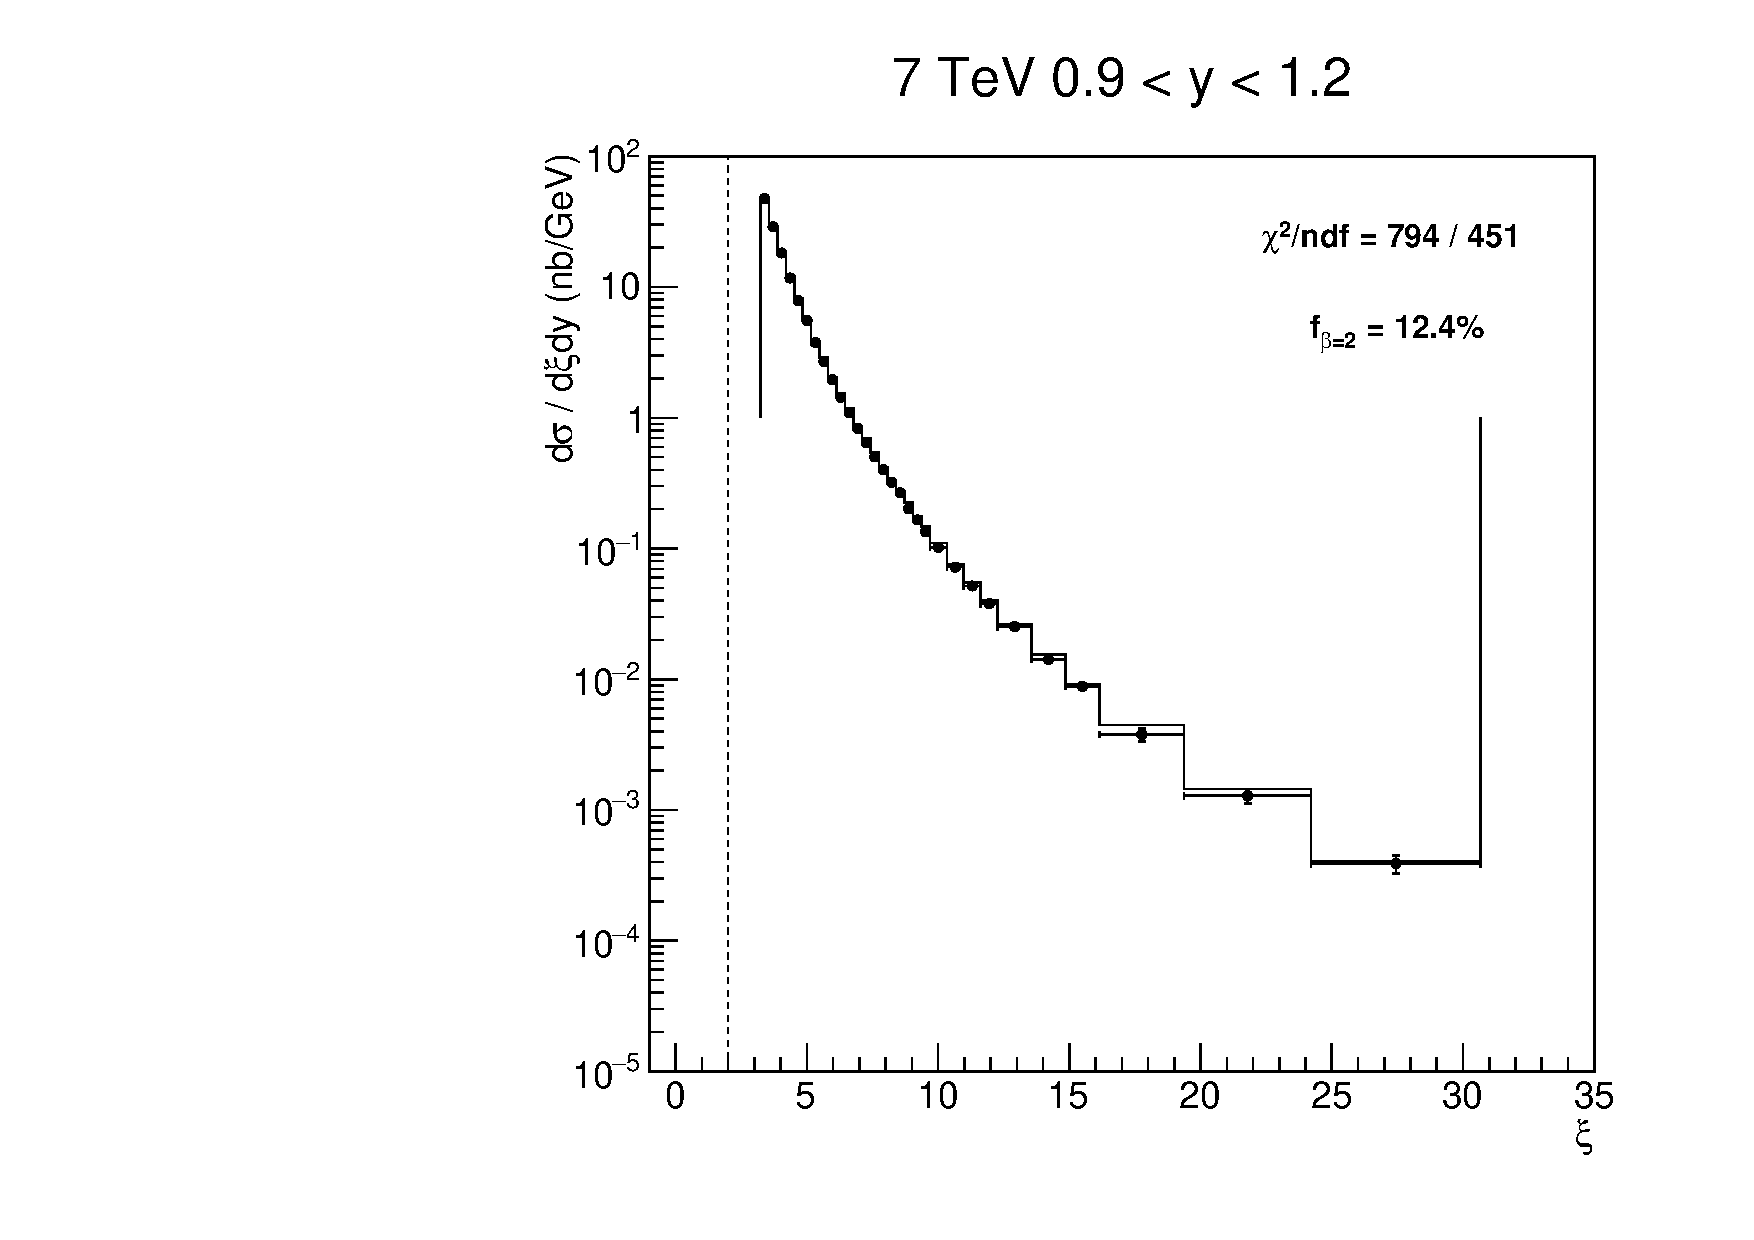
\includegraphics[width = 0.4\textwidth]{xi_7_y4.pdf}
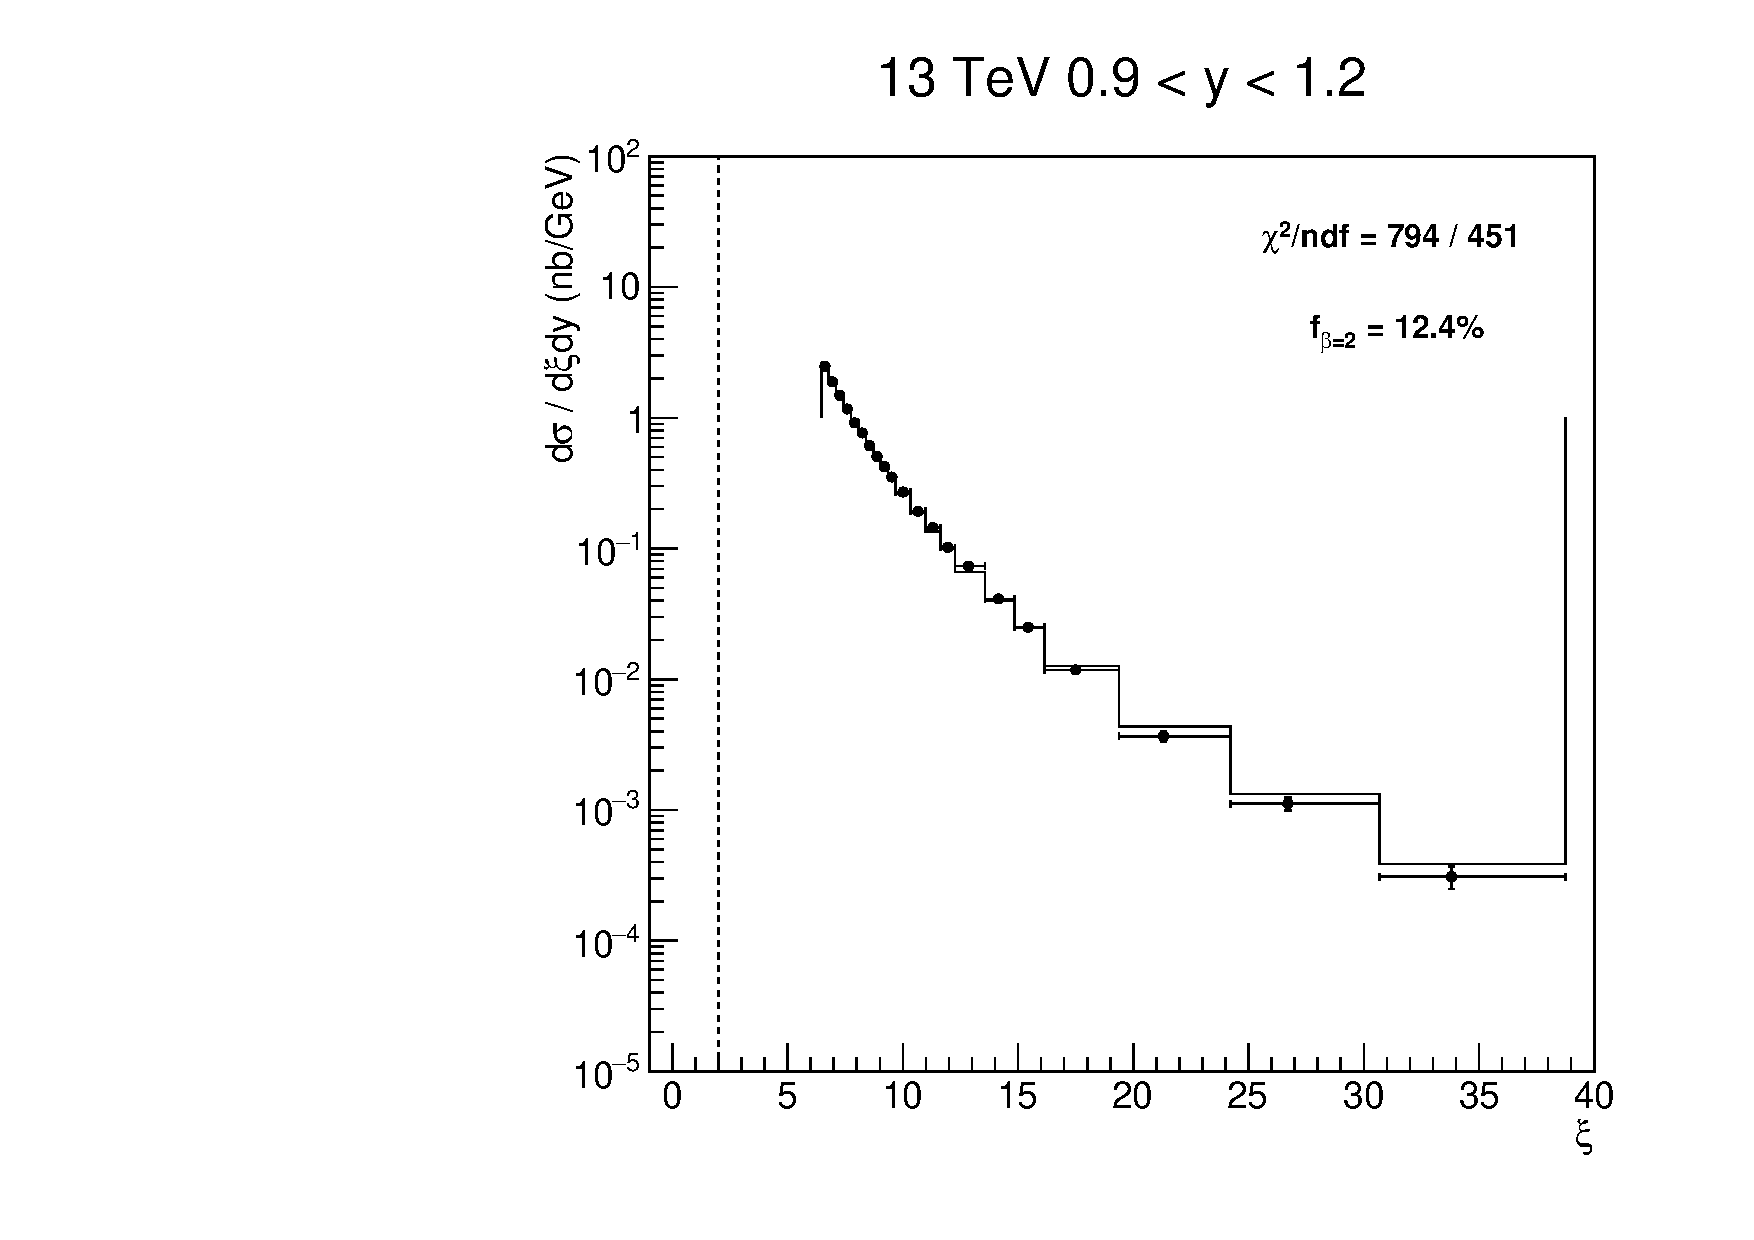
\includegraphics[width = 0.4\textwidth]{xi_13_y4.pdf}

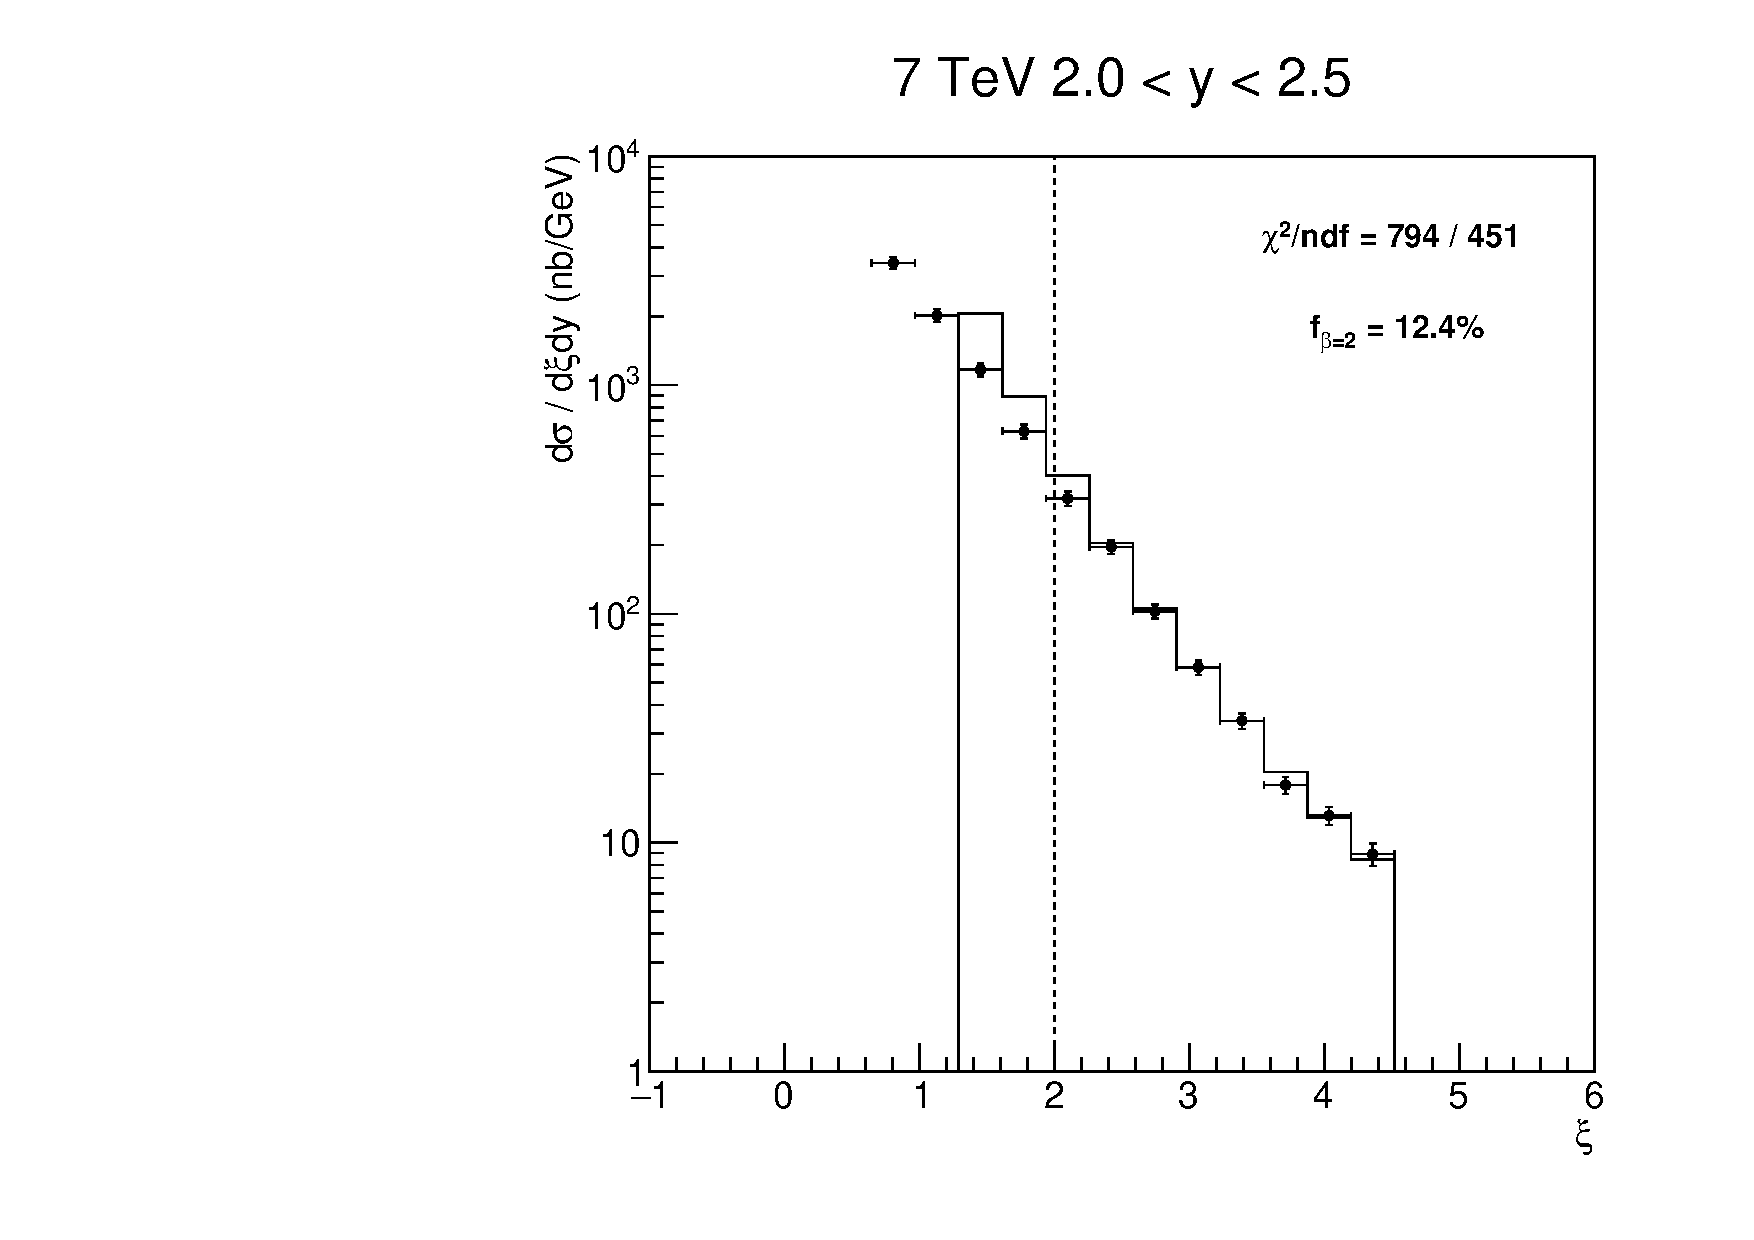
\includegraphics[width = 0.4\textwidth]{xi_7_y5.pdf}
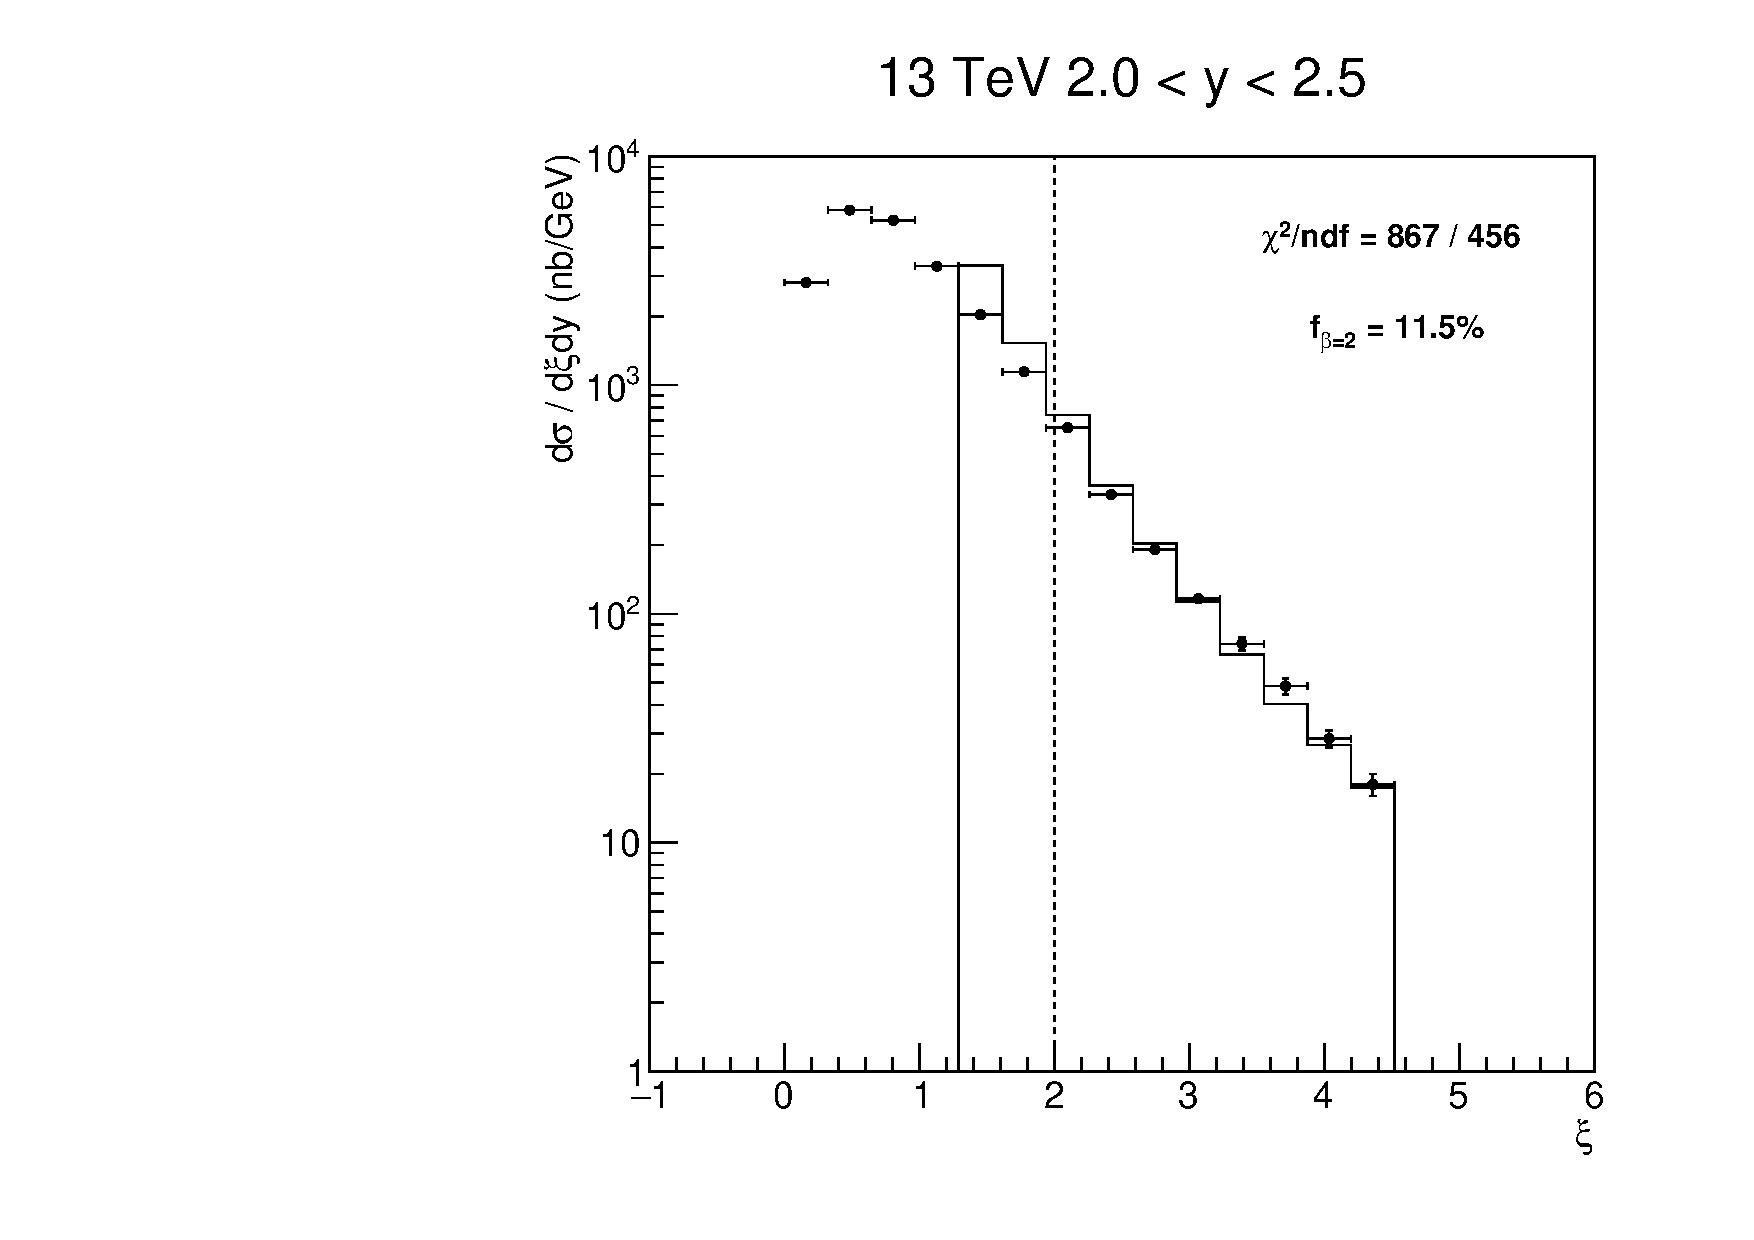
\includegraphics[width = 0.4\textwidth]{xi_13_y5.pdf}

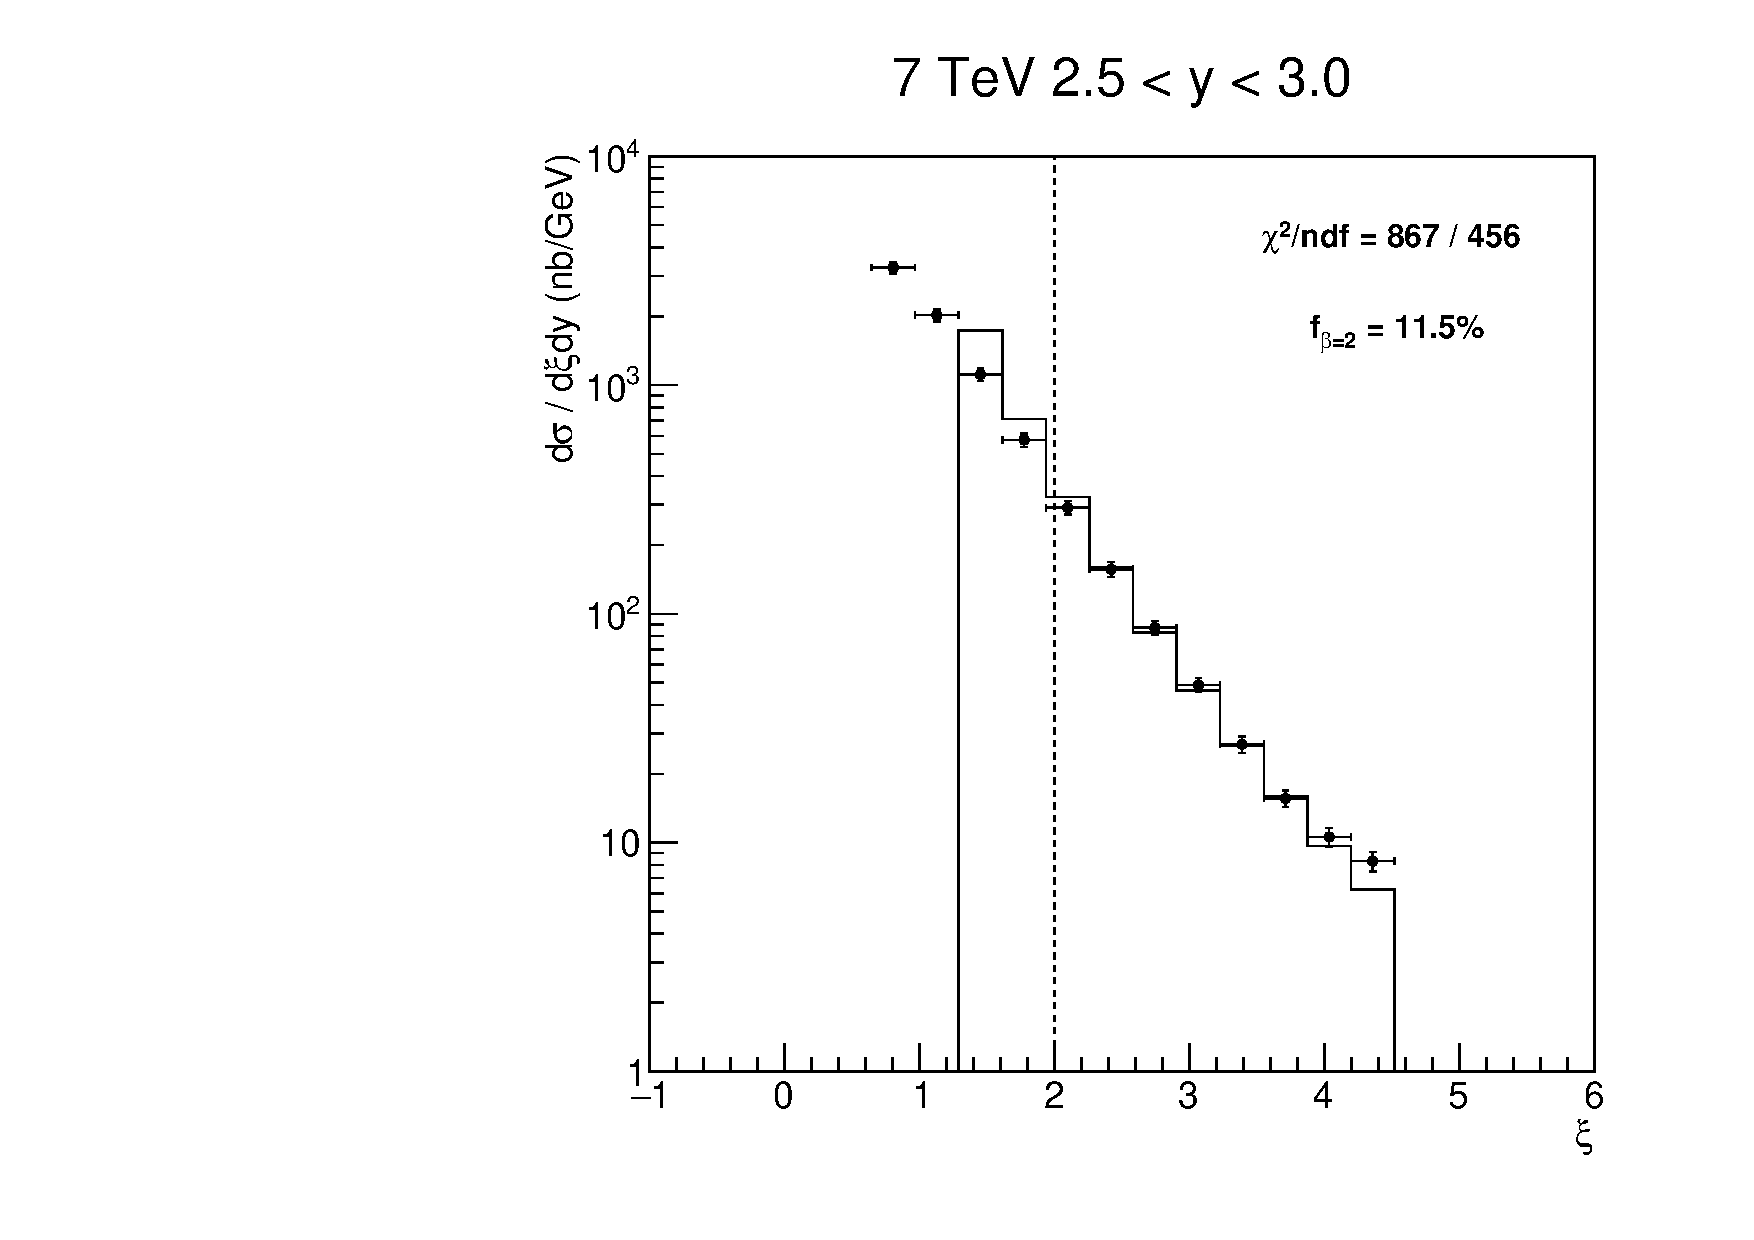
\includegraphics[width = 0.4\textwidth]{xi_7_y6.pdf}
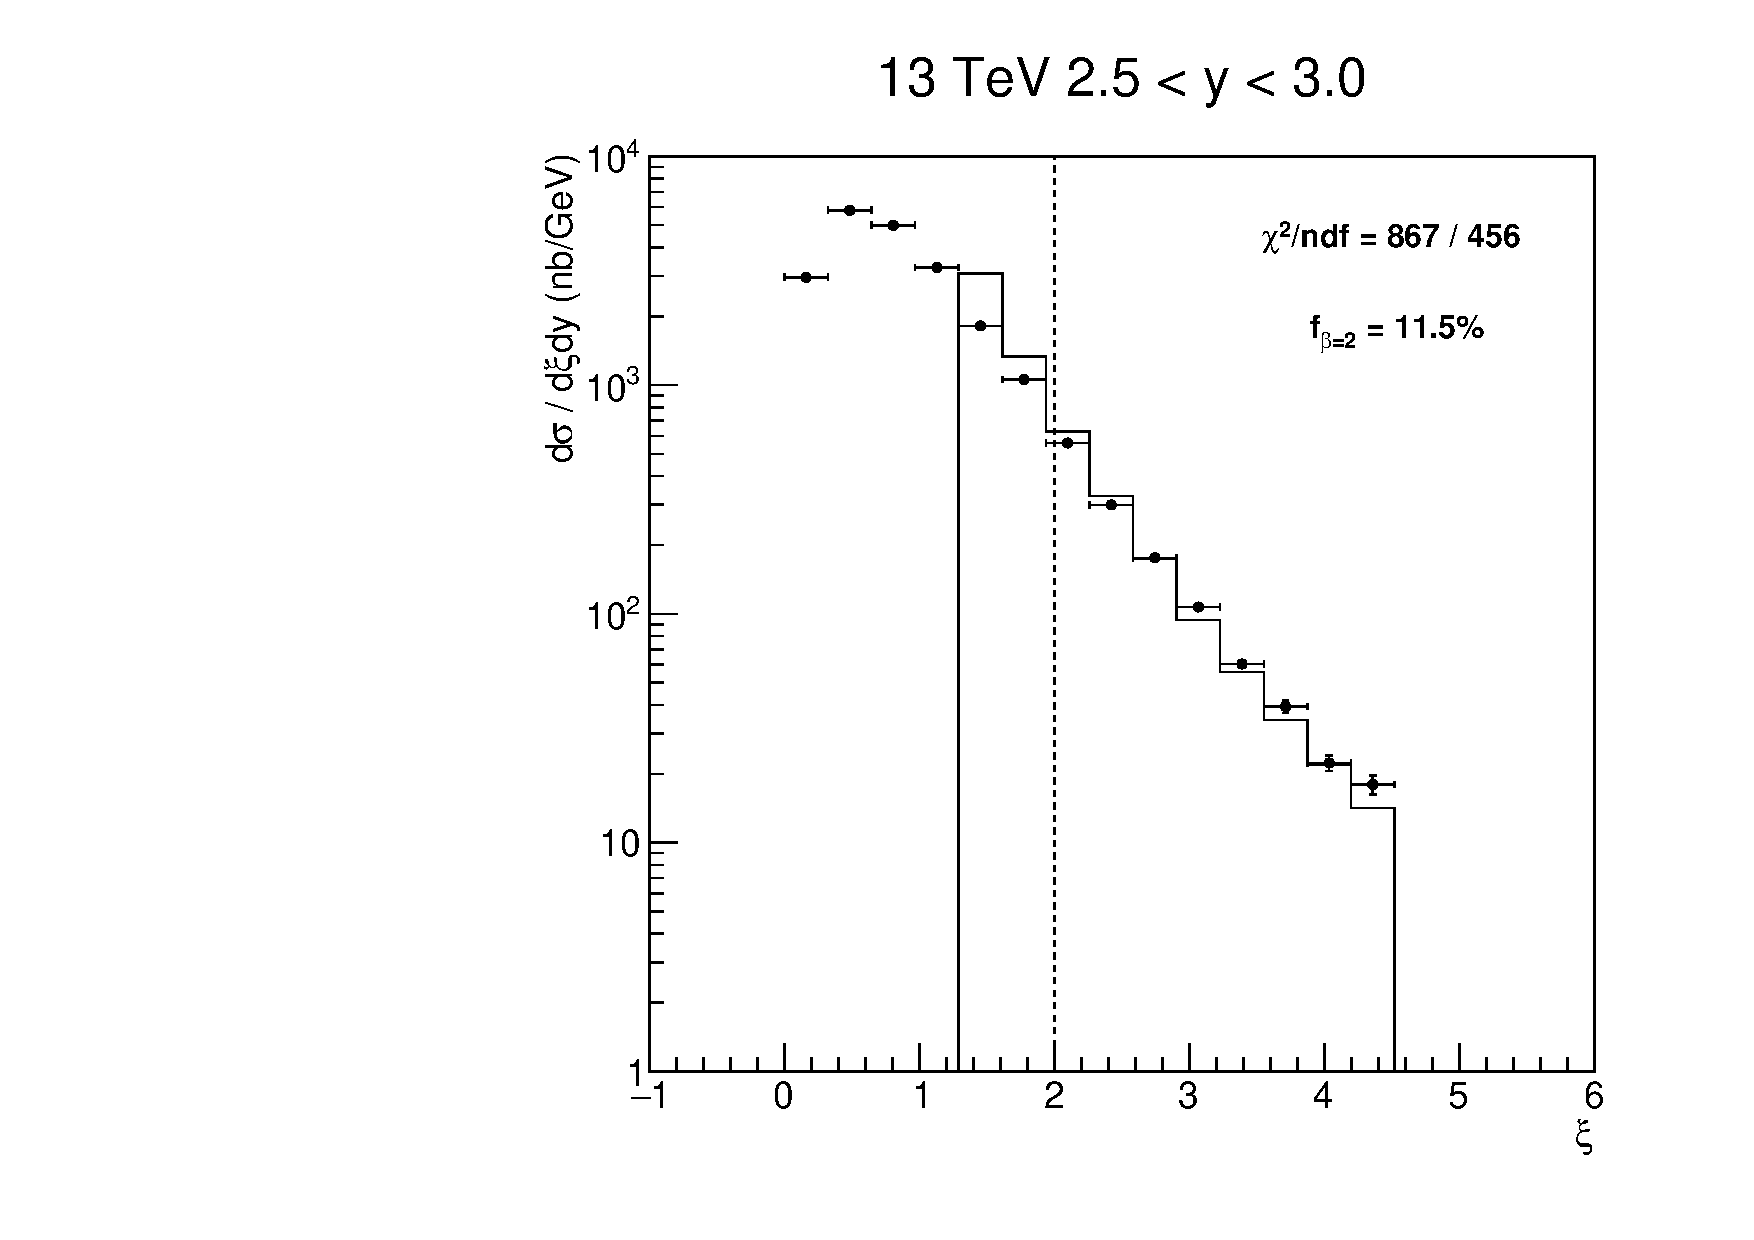
\includegraphics[width = 0.4\textwidth]{xi_13_y6.pdf}
\caption{Comparison between MC $\xi$ distribution and data points in the first three $y$ bins of the data, for 7 TeV (left) and 13 TeV (right).}\label{f:xi_comp_2}
\end{figure}

\clearpage

\begin{figure}[h!]
\centering
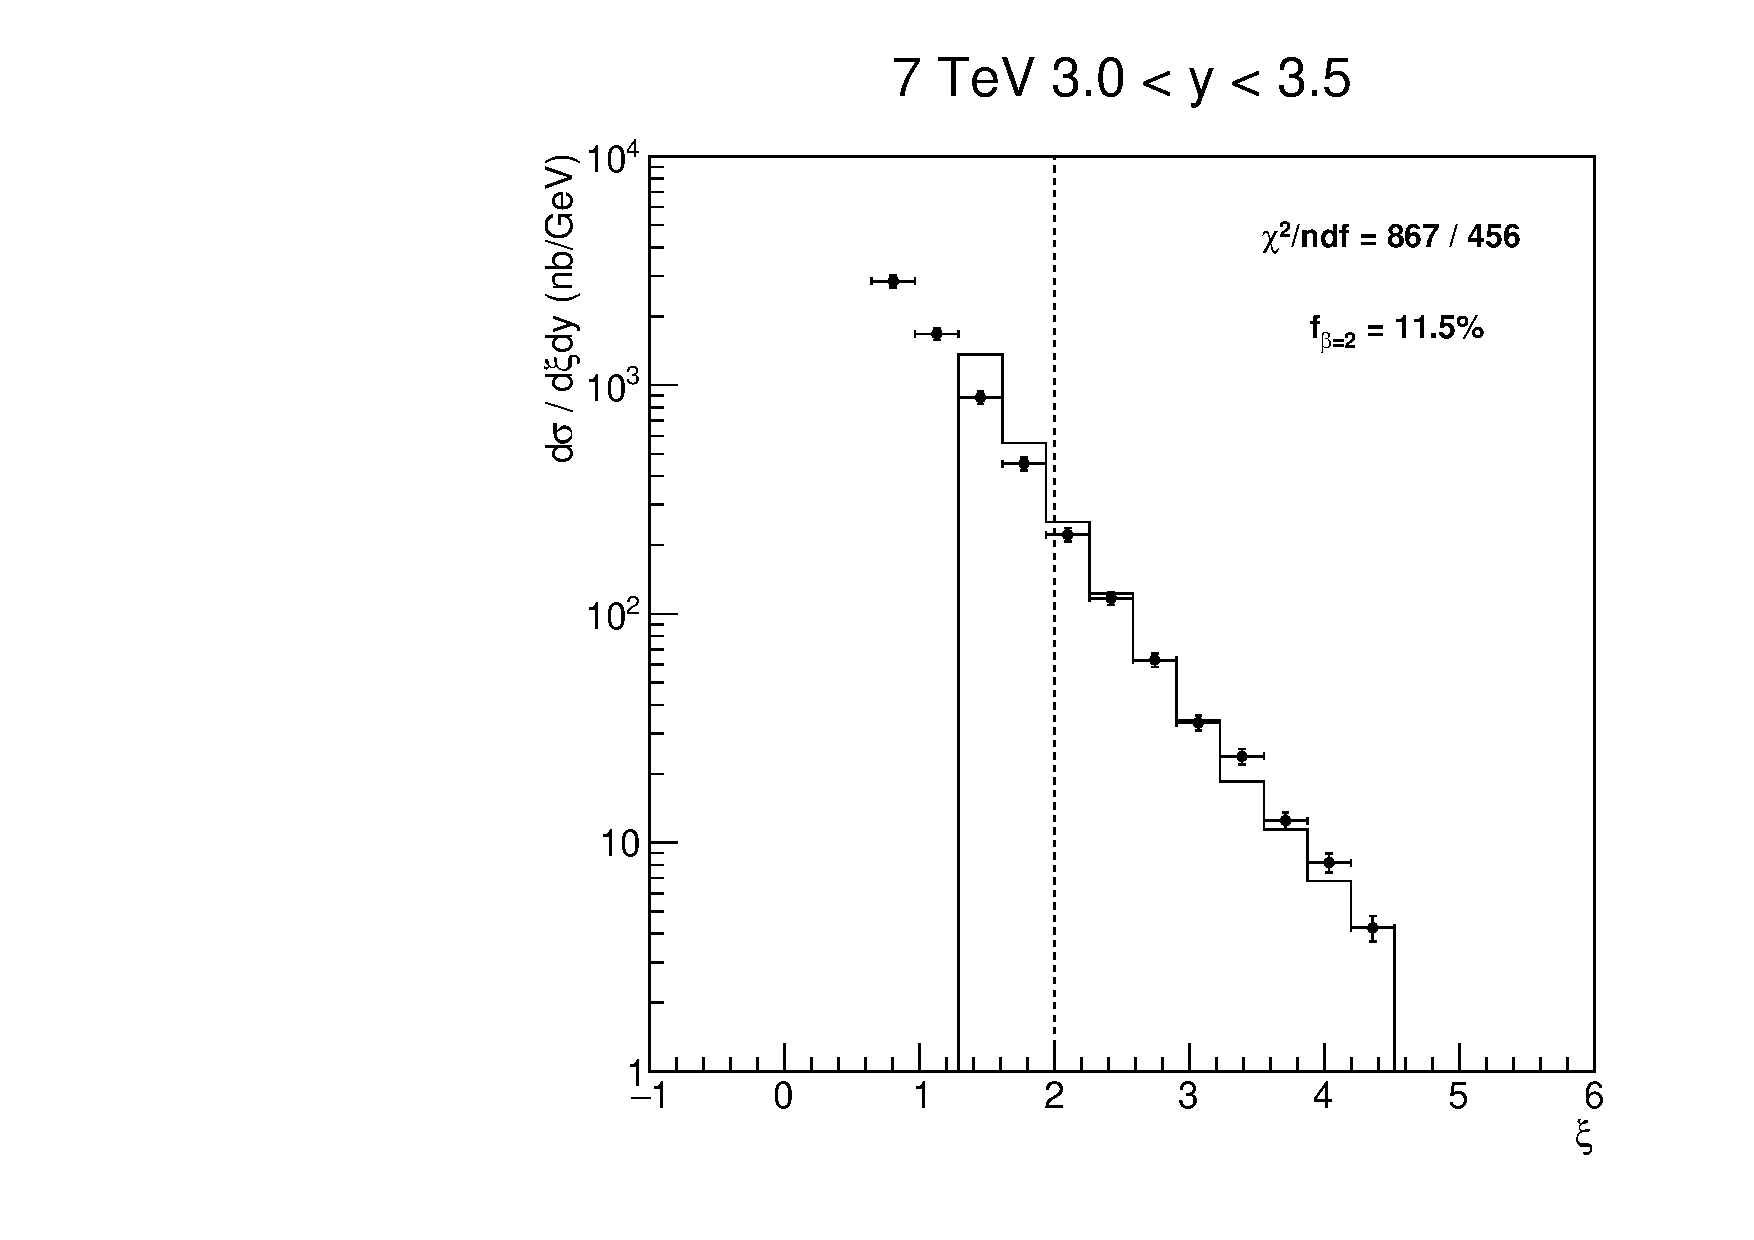
\includegraphics[width = 0.4\textwidth]{xi_7_y7.pdf}
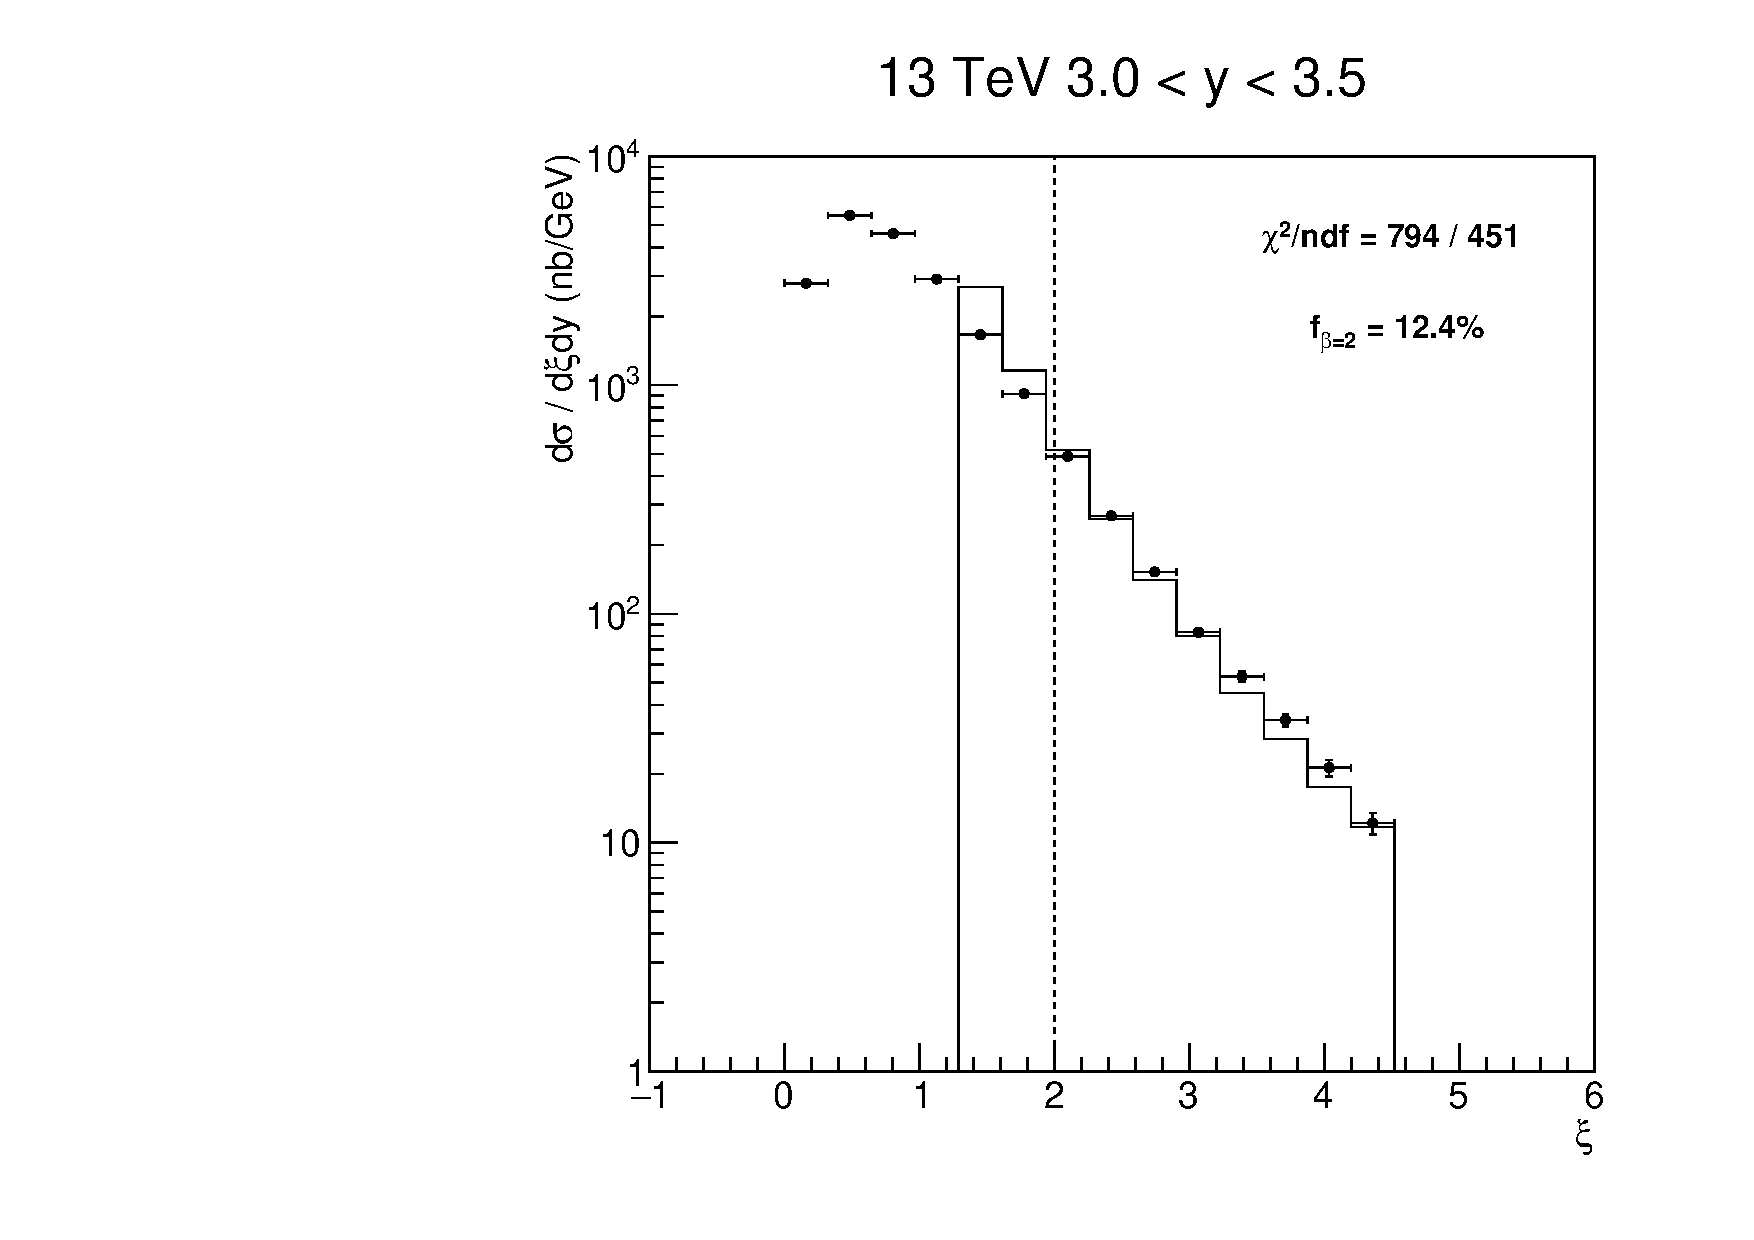
\includegraphics[width = 0.4\textwidth]{xi_13_y7.pdf}

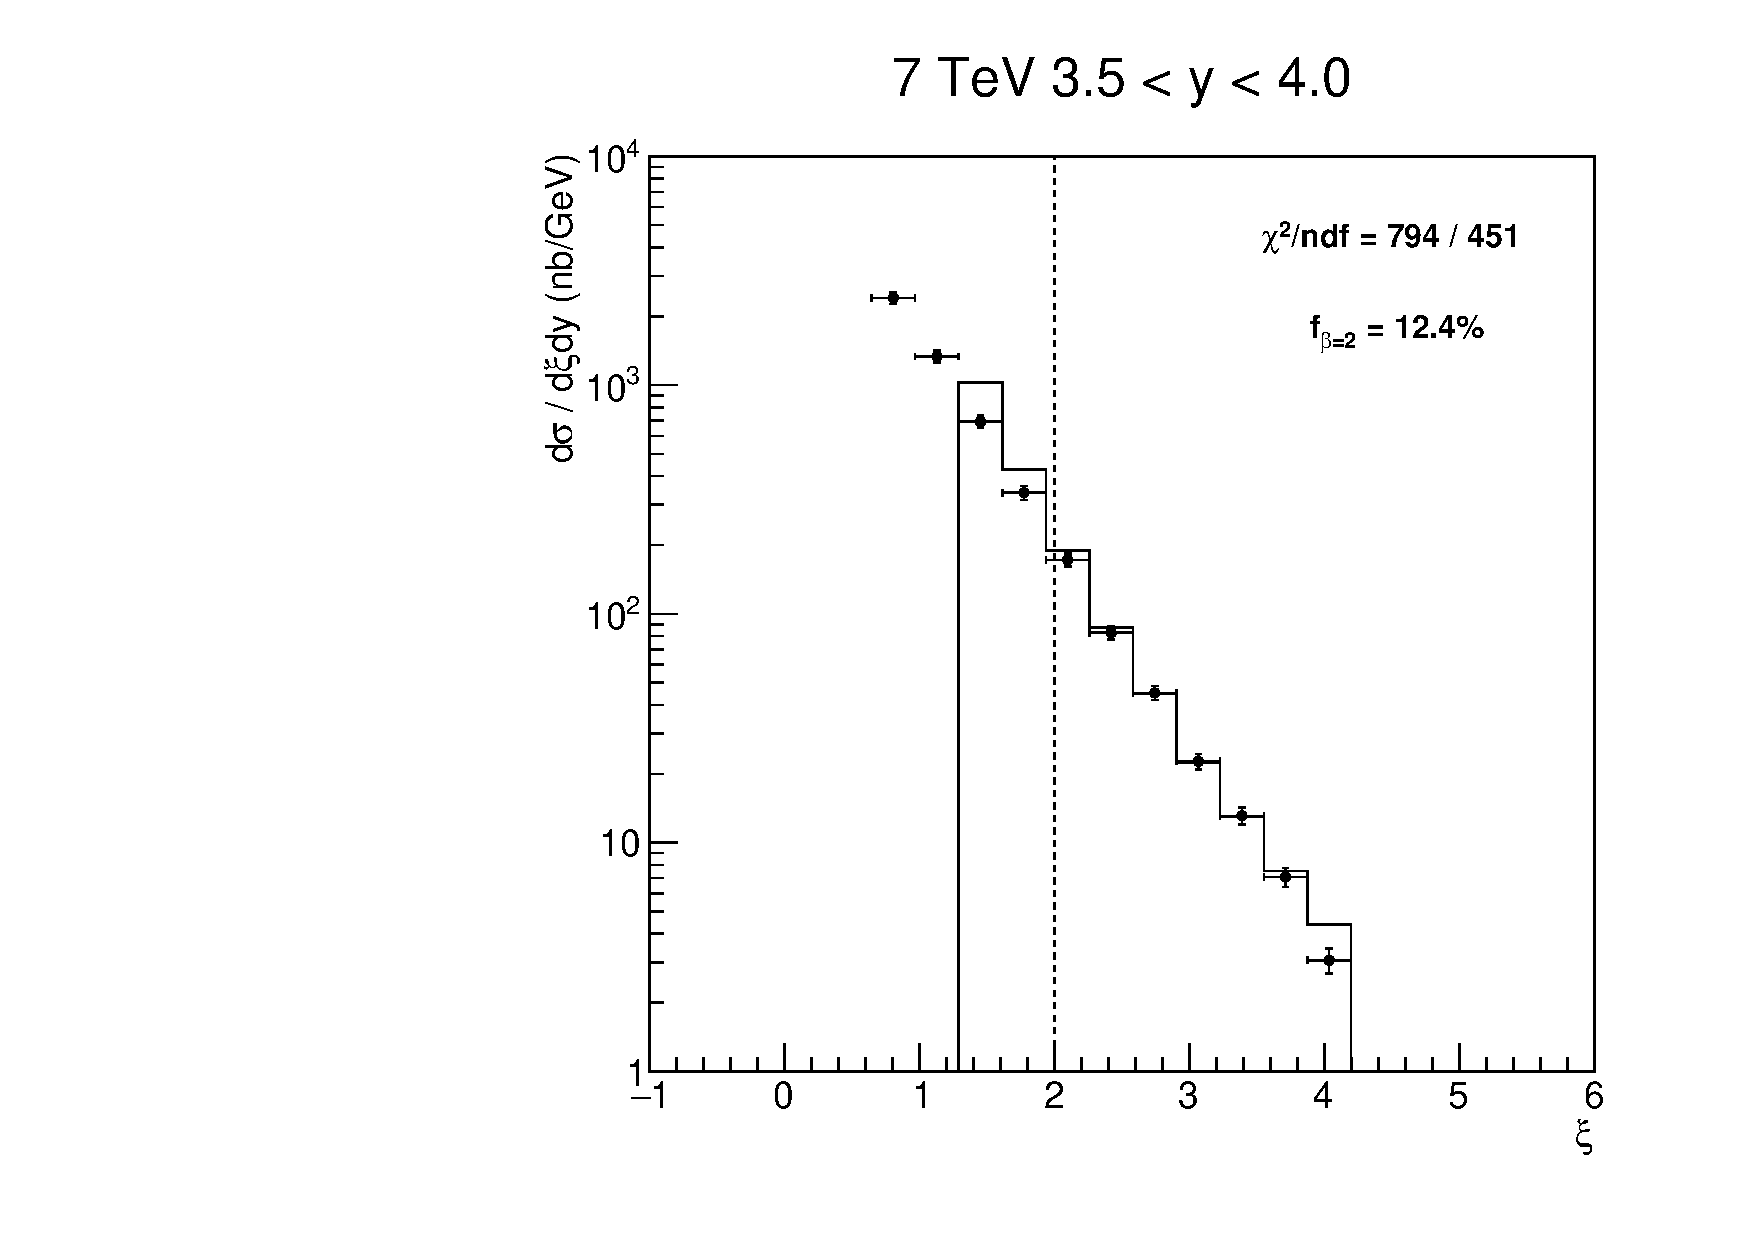
\includegraphics[width = 0.4\textwidth]{xi_7_y8.pdf}
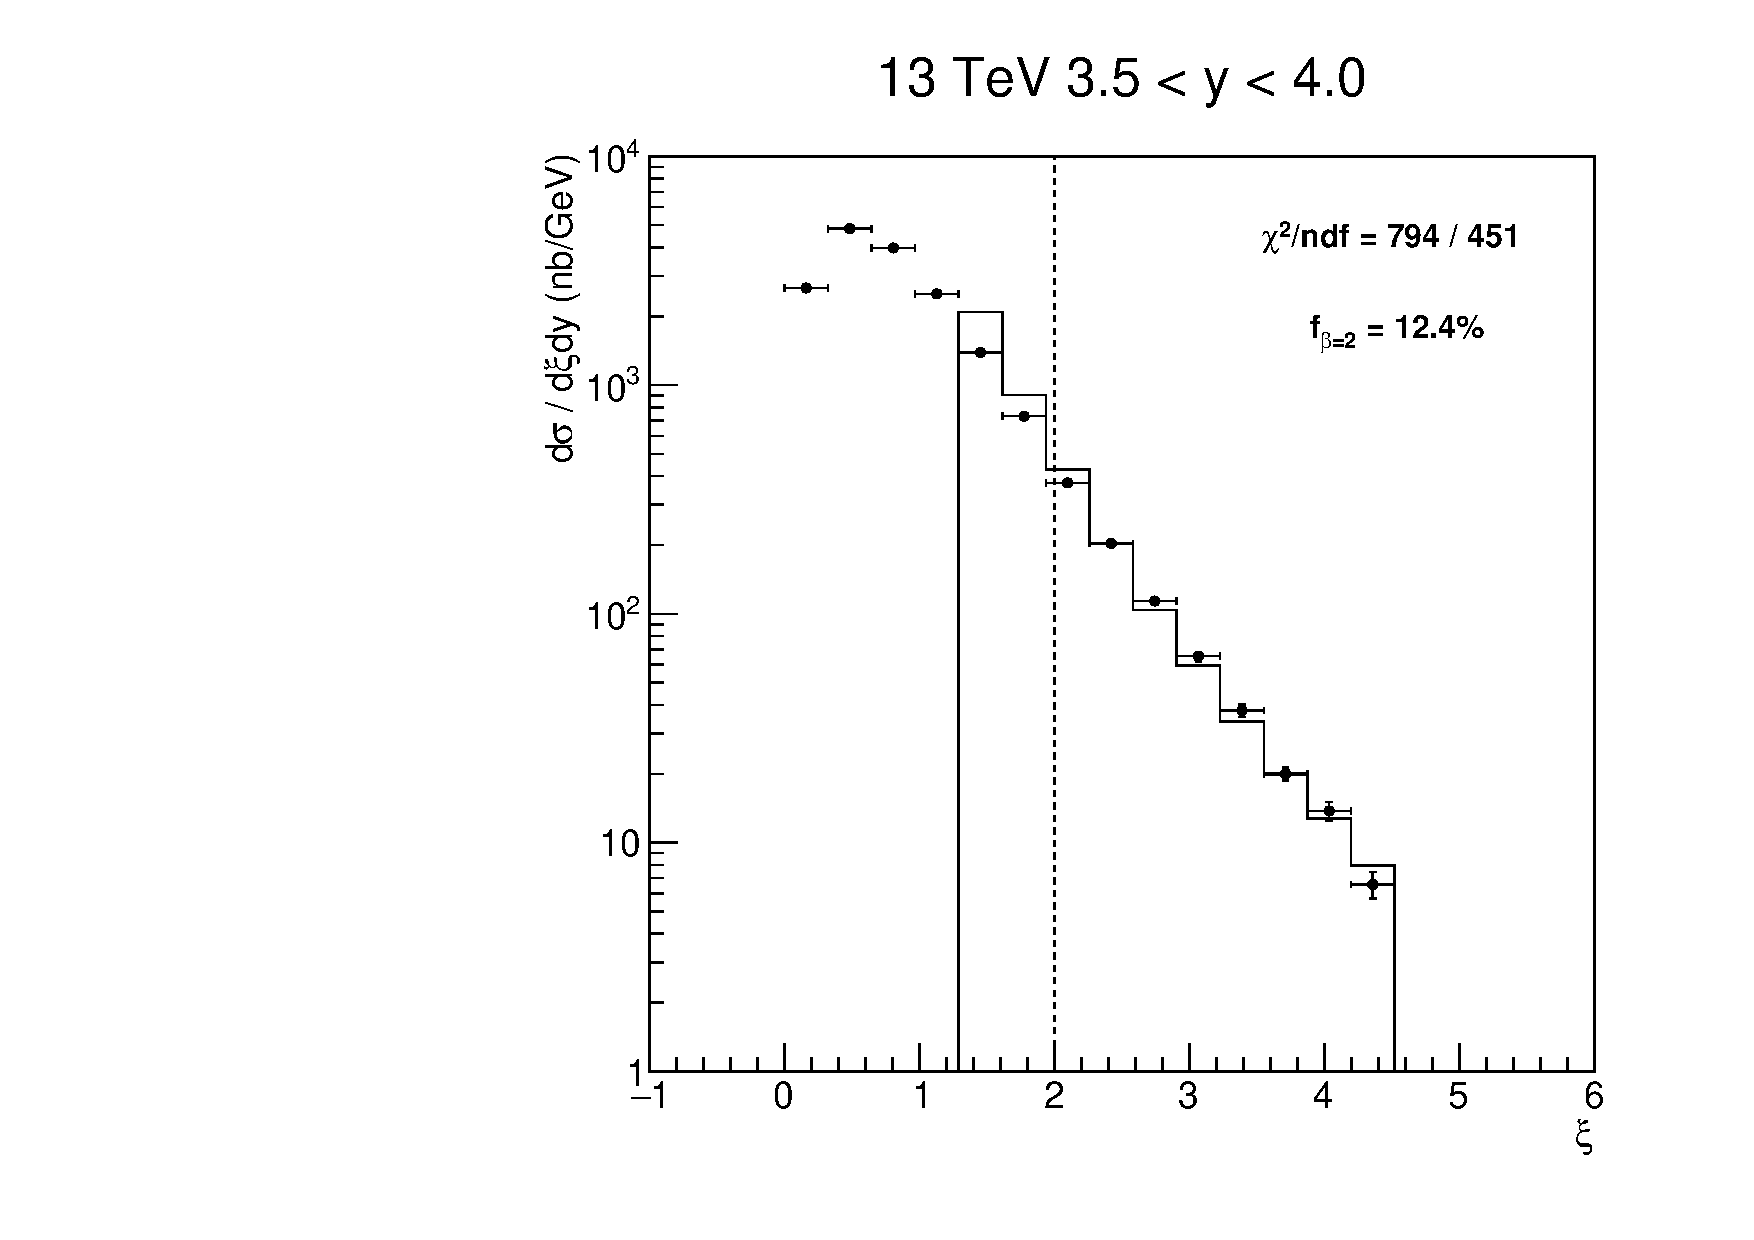
\includegraphics[width = 0.4\textwidth]{xi_13_y8.pdf}

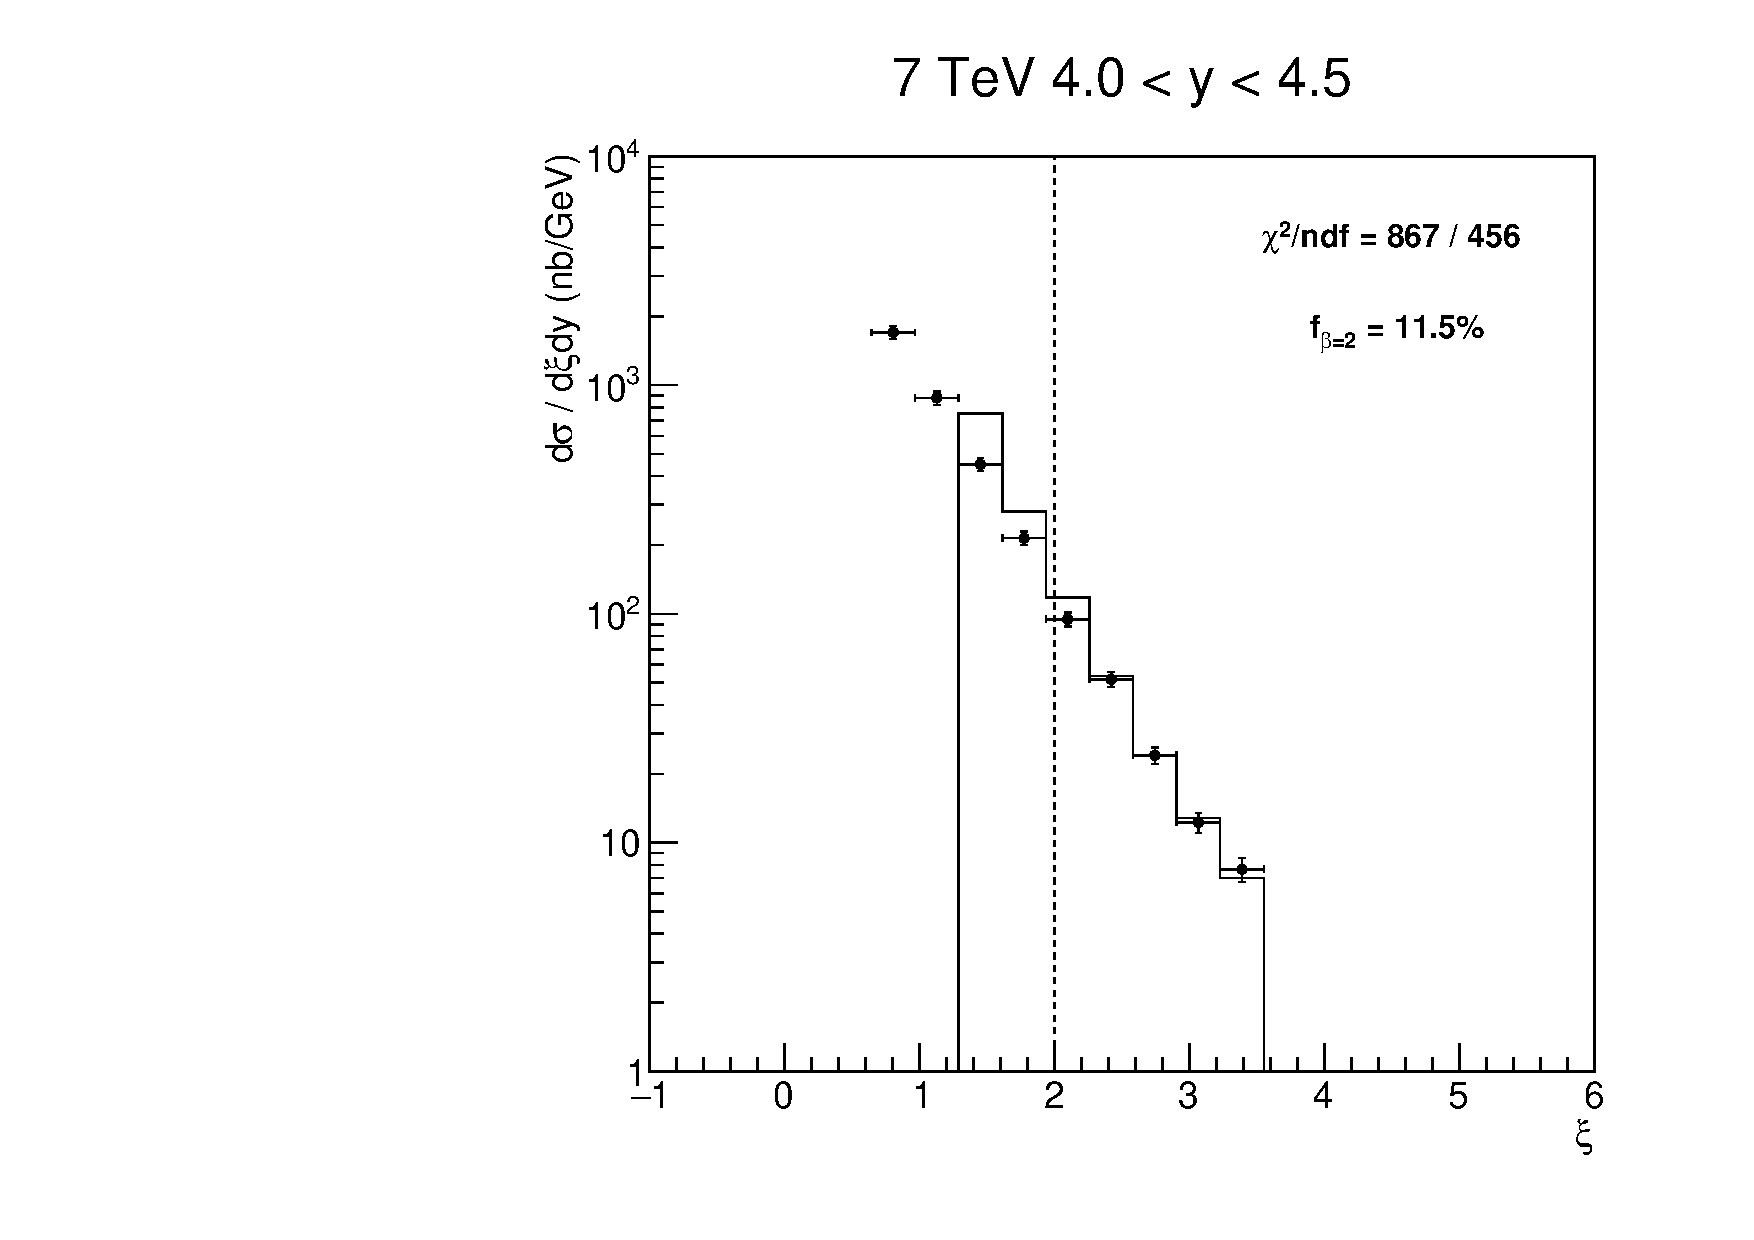
\includegraphics[width = 0.4\textwidth]{xi_7_y9.pdf}
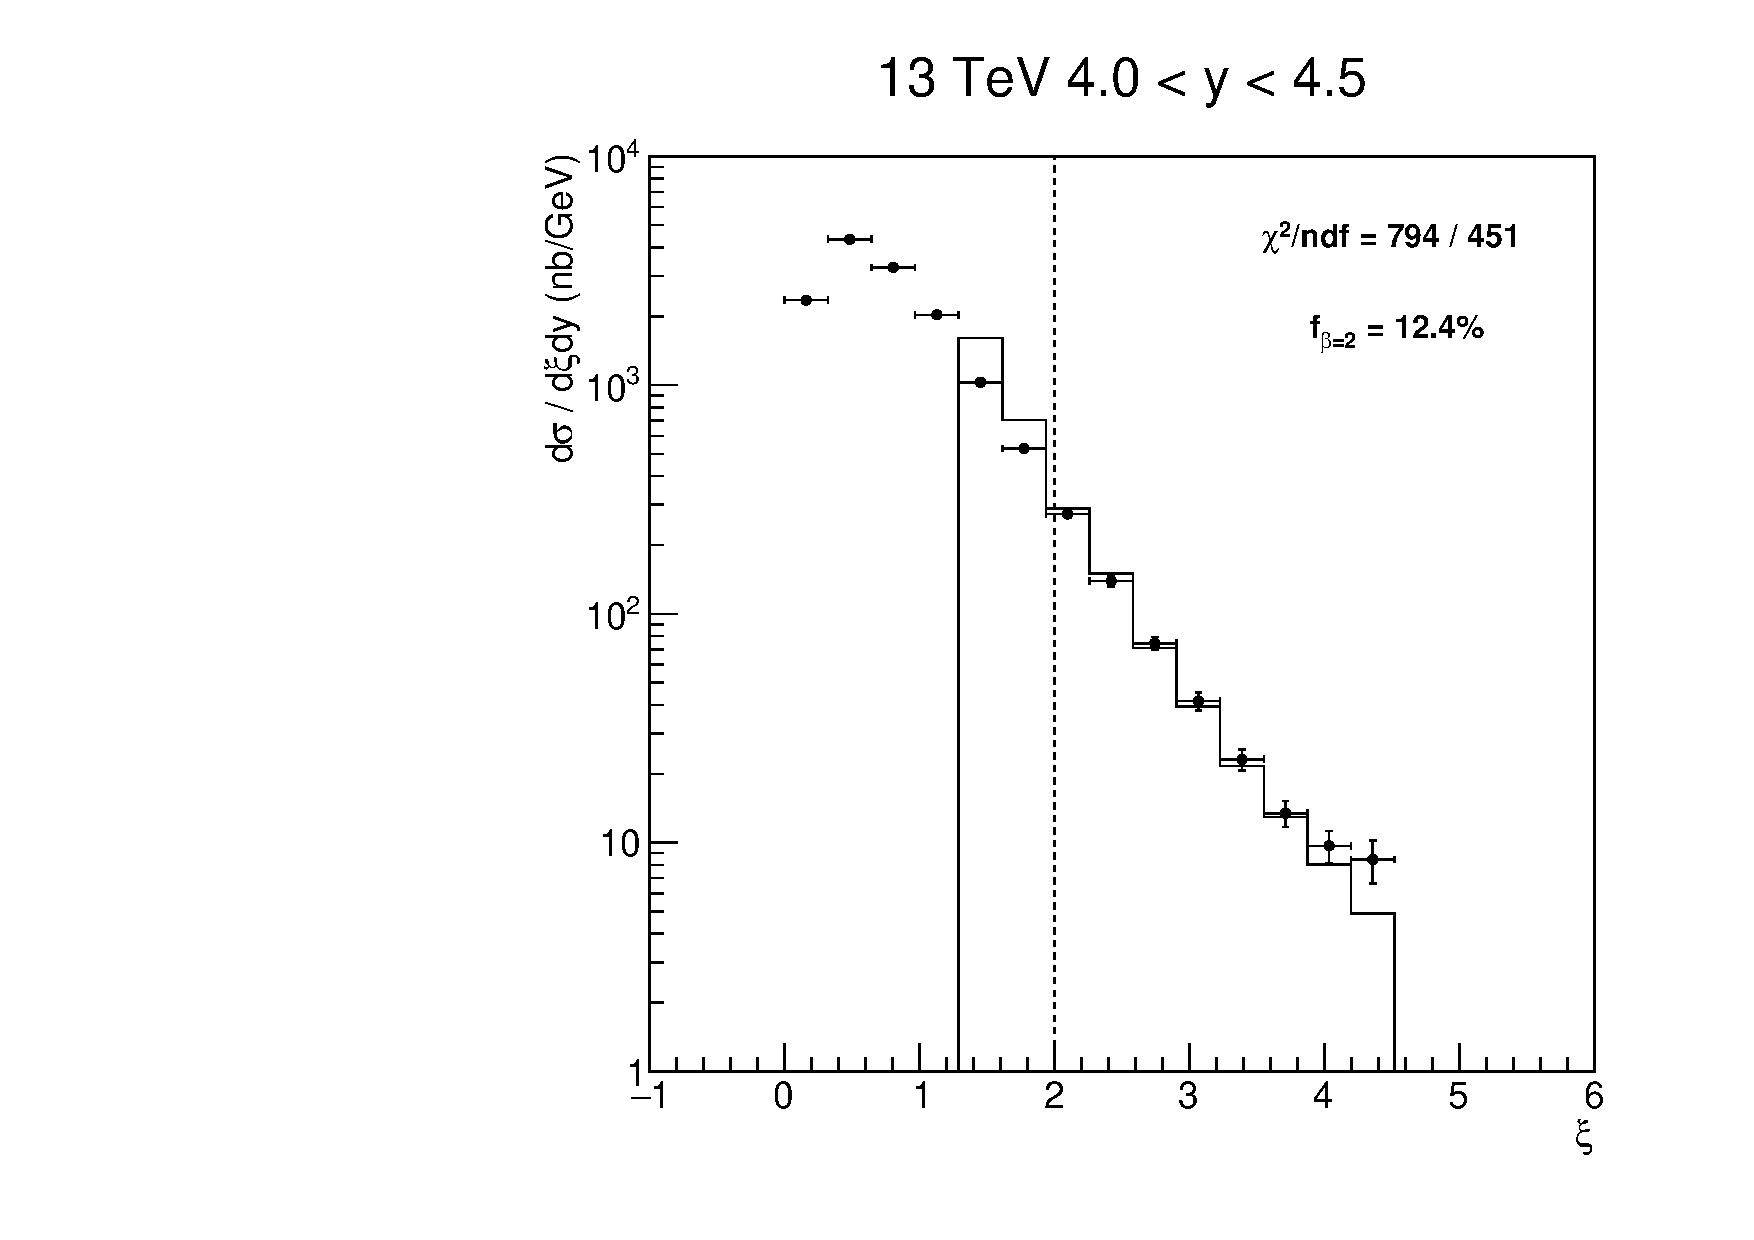
\includegraphics[width = 0.4\textwidth]{xi_13_y9.pdf}
\caption{Comparison between MC $\xi$ distribution and data points in the last three $y$ bins of the data, for 7 TeV (left) and 13 TeV (right).}\label{f:xi_comp_3}
\end{figure}


\end{document}